\documentclass[conference]{IEEEtran}
% Preamble for the English IEEE ICRA / IROS conference submission draft (P2, P3).
% Requires: \documentclass[conference]{IEEEtran} before % Preamble for the English IEEE ICRA / IROS conference submission draft (P2, P3).
% Requires: \documentclass[conference]{IEEEtran} before % Preamble for the English IEEE ICRA / IROS conference submission draft (P2, P3).
% Requires: \documentclass[conference]{IEEEtran} before \input{preamble}.
\usepackage{amsmath,amssymb,amsthm,mathtools}
\usepackage{graphicx}
\usepackage{booktabs,multirow,array,tabularx}
\usepackage[caption=false]{subfig}
\usepackage{algorithm}
\usepackage{algpseudocode}
\usepackage{url}
\usepackage{textcomp}
\usepackage{microtype}
\usepackage{xcolor}
\usepackage{bm}
\usepackage{balance}
\raggedbottom
\usepackage[hidelinks]{hyperref}

\graphicspath{{figures/}}

% Independent counters for lemmas / theorems / propositions so that the numbering
% matches paper/draft.md (Lemma 1, Theorem 1, Lemmas 2-5, Theorems 2-3, Props 1-3).
\newtheorem{theorem}{Theorem}
\newtheorem{lemma}{Lemma}
\newtheorem{proposition}{Proposition}
\newtheorem{corollary}{Corollary}
\theoremstyle{definition}
\newtheorem{definition}{Definition}
\newtheorem{assumption}{Assumption}
\newtheorem{example}{Example}
\theoremstyle{remark}
\newtheorem{remark}[theorem]{Remark}

\newcommand{\R}{\mathbb{R}}
\newcommand{\Sm}{\mathbb{S}}
\newcommand{\bq}{\mathbf{q}}
\newcommand{\bt}{\mathbf{t}}
\newcommand{\bx}{\mathbf{x}}
\newcommand{\bu}{\mathbf{u}}
\newcommand{\br}{\mathbf{r}}
\newcommand{\bM}{\mathbf{M}}
\newcommand{\bD}{\mathbf{D}}
\newcommand{\bG}{\mathbf{G}}
\newcommand{\bH}{\mathbf{H}}
\newcommand{\bE}{\mathbf{E}}
\newcommand{\bJ}{\mathbf{J}}
\newcommand{\vtwo}{v_2}
\newcommand{\tr}{\operatorname{tr}}
\newcommand{\rank}{\operatorname{rank}}
\newcommand{\diag}{\operatorname{diag}}
\newcommand{\Proj}{\operatorname{Proj}}
\newcommand{\argmin}{\operatorname*{arg\,min}}

\newcommand{\pend}[1]{\textcolor{red}{[#1]}}
\newcommand{\ev}[1]{\emph{#1}}
.
\usepackage{amsmath,amssymb,amsthm,mathtools}
\usepackage{graphicx}
\usepackage{booktabs,multirow,array,tabularx}
\usepackage[caption=false]{subfig}
\usepackage{algorithm}
\usepackage{algpseudocode}
\usepackage{url}
\usepackage{textcomp}
\usepackage{microtype}
\usepackage{xcolor}
\usepackage{bm}
\usepackage{balance}
\raggedbottom
\usepackage[hidelinks]{hyperref}

\graphicspath{{figures/}}

% Independent counters for lemmas / theorems / propositions so that the numbering
% matches paper/draft.md (Lemma 1, Theorem 1, Lemmas 2-5, Theorems 2-3, Props 1-3).
\newtheorem{theorem}{Theorem}
\newtheorem{lemma}{Lemma}
\newtheorem{proposition}{Proposition}
\newtheorem{corollary}{Corollary}
\theoremstyle{definition}
\newtheorem{definition}{Definition}
\newtheorem{assumption}{Assumption}
\newtheorem{example}{Example}
\theoremstyle{remark}
\newtheorem{remark}[theorem]{Remark}

\newcommand{\R}{\mathbb{R}}
\newcommand{\Sm}{\mathbb{S}}
\newcommand{\bq}{\mathbf{q}}
\newcommand{\bt}{\mathbf{t}}
\newcommand{\bx}{\mathbf{x}}
\newcommand{\bu}{\mathbf{u}}
\newcommand{\br}{\mathbf{r}}
\newcommand{\bM}{\mathbf{M}}
\newcommand{\bD}{\mathbf{D}}
\newcommand{\bG}{\mathbf{G}}
\newcommand{\bH}{\mathbf{H}}
\newcommand{\bE}{\mathbf{E}}
\newcommand{\bJ}{\mathbf{J}}
\newcommand{\vtwo}{v_2}
\newcommand{\tr}{\operatorname{tr}}
\newcommand{\rank}{\operatorname{rank}}
\newcommand{\diag}{\operatorname{diag}}
\newcommand{\Proj}{\operatorname{Proj}}
\newcommand{\argmin}{\operatorname*{arg\,min}}

\newcommand{\pend}[1]{\textcolor{red}{[#1]}}
\newcommand{\ev}[1]{\emph{#1}}
.
\usepackage{amsmath,amssymb,amsthm,mathtools}
\usepackage{graphicx}
\usepackage{booktabs,multirow,array,tabularx}
\usepackage[caption=false]{subfig}
\usepackage{algorithm}
\usepackage{algpseudocode}
\usepackage{url}
\usepackage{textcomp}
\usepackage{microtype}
\usepackage{xcolor}
\usepackage{bm}
\usepackage{balance}
\raggedbottom
\usepackage[hidelinks]{hyperref}

\graphicspath{{figures/}}

% Independent counters for lemmas / theorems / propositions so that the numbering
% matches paper/draft.md (Lemma 1, Theorem 1, Lemmas 2-5, Theorems 2-3, Props 1-3).
\newtheorem{theorem}{Theorem}
\newtheorem{lemma}{Lemma}
\newtheorem{proposition}{Proposition}
\newtheorem{corollary}{Corollary}
\theoremstyle{definition}
\newtheorem{definition}{Definition}
\newtheorem{assumption}{Assumption}
\newtheorem{example}{Example}
\theoremstyle{remark}
\newtheorem{remark}[theorem]{Remark}

\newcommand{\R}{\mathbb{R}}
\newcommand{\Sm}{\mathbb{S}}
\newcommand{\bq}{\mathbf{q}}
\newcommand{\bt}{\mathbf{t}}
\newcommand{\bx}{\mathbf{x}}
\newcommand{\bu}{\mathbf{u}}
\newcommand{\br}{\mathbf{r}}
\newcommand{\bM}{\mathbf{M}}
\newcommand{\bD}{\mathbf{D}}
\newcommand{\bG}{\mathbf{G}}
\newcommand{\bH}{\mathbf{H}}
\newcommand{\bE}{\mathbf{E}}
\newcommand{\bJ}{\mathbf{J}}
\newcommand{\vtwo}{v_2}
\newcommand{\tr}{\operatorname{tr}}
\newcommand{\rank}{\operatorname{rank}}
\newcommand{\diag}{\operatorname{diag}}
\newcommand{\Proj}{\operatorname{Proj}}
\newcommand{\argmin}{\operatorname*{arg\,min}}

\newcommand{\pend}[1]{\textcolor{red}{[#1]}}
\newcommand{\ev}[1]{\emph{#1}}

\begin{document}

\title{Robust-QPEPLayer: Curvature-Corrected Implicit Differentiation for RANSAC-Free Robust Pose Estimation}

\author{\IEEEauthorblockN{First Author}
\IEEEauthorblockA{Department, Institution\\
City, Country\\
Email address}}

\maketitle

\begin{abstract}
Differentiable pose-estimation layers promise end-to-end learning through geometric optimization,
but are fragile under outliers: the state of the art either wraps a non-differentiable RANSAC
front-end around a certifiable solver, or differentiates a local robust $M$-estimator with frozen
or unrolled weights. We present \textbf{Robust-QPEPLayer}, a RANSAC-free differentiable pose layer
combining Black--Rangarajan (BR) duality, graduated non-convexity (GNC), and a constant-size
quaternion pose solver (QPEP). Its forward pass alternates a closed-form weight update with a
globally solved weighted QPEP (in the scalar-weight 3D--3D tables, its closed-form $4\times4$
specialization), so rotation stays four-dimensional (three on the tangent space) and $N$ enters
only through $O(N)$ accumulation; its backward pass differentiates the robust fixed point exactly
with a $6\times6$ system and $O(1)$ memory in the GNC iterations. We prove an exact BR dual for the
Geman--McClure kernel, that a GNC fixed point is stationary for the robust cost with the
redescending curvature correction equal to the Schur complement of the BR weight block, and the
exact Riemannian Hessian on $\mathbb{S}^3\times\mathbb{R}^3$, whose multiplier term
$-\lambda_{\mathrm{rob}}I$ is absent from the Euclidean formula and shifts the spectrum by $O(1)$.
We also prove a one-dimensional sign flip where frozen-weight IRLS-StopGrad has the opposite
derivative sign, and a per-observation $O(\|\mathbf{r}_i\|^{-4})$ gradient bound distinct from
forward robustness. GNC is not global, coherent majority outliers can make the robust optimum
wrong, and $H_{\mathrm{rob}}\succ0$ certifies local stability, not robustness. GNC-GM matches
fixed-1000 RANSAC through $70\%$ random outliers at $22$--$32\times$ lower runtime, but is slower
than adaptive RANSAC at low outlier fractions (about $8\times$ faster at $70\%$). Exact IFT
matches finite differences at $3$--$5\times10^{-8}$; frozen weights give a boundary cosine of
$0.234$ and relative error $1.07$. On two daylight and two night-prefix UTIAS In-The-Dark runs
(hand-written SIFT+SGBM front-end, no training), GNC-GM reaches
$0.078$--$0.150^\circ/0.007$--$0.020$~m (sparse night $0.197^\circ$) with $79$--$97\%$ natural
inliers and $100\%$ success at $0.1$~m; full-night runs and end-to-end training remain untested.
Theseus-GM succeeds at $80/55/25\%$ for $30/50/70\%$ outliers versus GNC's $100\%$; a KITTI stereo
fallback is rotation-positive and translation-negative.

\end{abstract}

\begin{IEEEkeywords}
robust pose estimation, differentiable optimization, Black--Rangarajan duality, graduated non-convexity, implicit differentiation.
\end{IEEEkeywords}

\section{Introduction}

Optimization layers are now standard in differentiable robotics and vision: a geometric problem is
solved in the forward pass, and implicit differentiation of its optimality conditions provides
gradients to an upstream network \cite{holmes2025sdpr,pineda2022theseus,chen2020bpn}. For pose
estimation the difficulty is non-convexity: local solvers converge to \emph{a} stationary point
whose gradient is generally not the gradient of the global pose. SDPRLayers
\cite{holmes2025sdpr} solves a convex semidefinite relaxation, certifies rank-one optimality, and
differentiates the original KKT system there; QPEP \cite{wu2022qpep} eliminates translation,
enumerates all stationary points of a quartic system with a Gr\"obner basis, and returns the
algebraically global optimum. Both are global in the forward pass, but neither is robust: SDPRLayers'
real-data experiments wrap the layer in RANSAC \cite{fischler1981ransac} and train on clean samples,
and a robust SDP with per-correspondence binary variables lifts a $10\times10$ matrix to
$(10+9N)\times(10+9N)$ \cite{holmes2025sdpr}.

This paper asks: \emph{can we obtain a differentiable pose layer that is robust to gross outliers,
has constant dimension in the number of correspondences, and differentiates the robust estimator
exactly rather than unrolling it or freezing its weights?} We answer with three ingredients:
\textbf{Black--Rangarajan duality} \cite{black1996br}, which turns a redescending $M$-estimator
into a joint optimization over the pose and one weight per correspondence; \textbf{graduated
non-convexity} \cite{yang2020gnc,yang2020teaser}, which anneals a convex surrogate towards the
redescending kernel; and \textbf{QPEP} \cite{wu2022qpep}, which solves each weighted subproblem
globally in a fixed number of variables. The combination is not new in spirit---GNC with a weighted
least-squares inner solver is standard in robust registration \cite{yang2020gnc,yang2020teaser}---but
the \emph{differentiable} layer exposes a structure that, to our knowledge, has not been isolated:
the exact derivative of the robust fixed point contains a \emph{redescending curvature correction}
that is the Schur complement of the BR weight block, and on $\mathbb{S}^3$ it also contains a
\emph{constraint-multiplier term} that the Euclidean formula misses. Dropping either term makes
gradients wrong by a large factor, or even flips their sign for boundary outliers.

\subsection{Contributions}

\begin{enumerate}
\item \textbf{A constant-dimension robust forward pass with an exact dual.} The BR dual of the
  Geman--McClure (GM) kernel is exact for every weight and annealing parameter, the optimal weight
  is the kernel derivative, and GNC-QPEP is a monotone block-coordinate descent whose limit points
  are coordinate-wise stationary (Lemma~\ref{lem:brdual}, Theorem~\ref{thm:gnc}). The inner
  weighted subproblem is solved globally; in the 3D--3D experiments it reduces to the closed-form
  $4\times4$ specialization.
\item \textbf{Exact fixed-point implicit differentiation with a curvature correction.} A GNC fixed
  point is a stationary point of the robust cost (Lemma~\ref{lem:fixedpoint}); the redescending
  correction is the eliminated weight block (Lemma~\ref{lem:schur}); and the exact Riemannian
  Hessian contains $-\lambda_{\mathrm{rob}}\diag(I_3,0_3)$ with the 3D--3D constant
  $\lambda_i=4\mathbf{u}_i^\top W_i\mathbf{r}_i$, \emph{not} $4e_i$ (Lemma~\ref{lem:hessian}).
  Dropping it changes the spectrum by $O(1)$.
\item \textbf{A rigorous sign-flip result and an $O(\|\mathbf{r}\|^{-4})$ gradient bound.} In a 1D
  location model, at a strict minimum with $H_{\mathrm{rob}}>0$, the exact derivative is
  $\lambda_\parallel(e_j)/H_{\mathrm{rob}}$ while the frozen-weight derivative is always positive;
  for $e_j>c^2/3$ the signs are strictly opposite (Proposition~\ref{prop:signflip}), and such a
  configuration exists for two well-separated observations (Proposition~\ref{prop:existence}). We
  also prove a per-observation $\|\partial z^*/\partial\mathbf{y}_i\|=O(\|\mathbf{r}_i\|^{-4})$
  bound under uniform invertibility, whereas the forward bias is only $O(\|\mathbf{r}_i\|^{-3})$
  (Proposition~\ref{prop:bound}).
\item \textbf{A unified kernel framework and an evaluation protocol.} We give the BR duals of
  GM, Cauchy, Welsch, and TLS, with structurally identical forward and backward passes
  (Appendix~\ref{app:kernel}), and evaluate on synthetic 3D--3D, ModelNet40/10, all eight official
  3DMatch test scenes, two KITTI raw drives, all 11 KITTI odometry sequences 00--10 (33 selected
  frames each), and four UTIAS In-The-Dark runs. Theseus and SDPRLayers serve as external baselines.
\end{enumerate}

The layer is complementary to Veronese-lifting and constrained-QPEP formulations: it uses neither
the $O(10)$ Veronese isomorphism nor inequality constraints, and shares only the QPEP inner solver.

\section{Related Work}
\label{sec:related}

\noindent\textbf{Certifiable and global pose layers.} SDPRLayers \cite{holmes2025sdpr} lifts a
homogeneous QCQP to a Shor SDP, certifies rank-one optimality, and differentiates the original KKT
system with an implicit-selection argument. Its guarantees are conditional on tightness; its
real-data pipeline uses RANSAC and clean samples, and its SDP grows with the number of variables.
QPEP \cite{wu2022qpep} eliminates translation, solves a quartic system by Gr\"obner basis, and
returns the algebraically global pose with a covariance, but has no gradient layer. We use the
scalar-weight $4\times4$ specialization of QPEP as a \emph{subroutine} and add a robust outer loop
and an exact backward; global optimality is confined to the inner weighted QPEP.

\noindent\textbf{Local differentiable optimization.} Theseus \cite{pineda2022theseus} provides
differentiable nonlinear least squares on Lie groups with implicit differentiation and direct loss
minimization. It supports robust kernels as soft costs, but its fixed point is a local stationary
point of the penalized objective, it does not expose the redescending curvature correction, and the
kernel is applied as a scalar weight rather than through a BR dual. BPnP \cite{chen2020bpn}
backpropagates through a PnP solver via the implicit function theorem and targets 3D--2D PnP. EPro-PnP
\cite{chen2022epropnp} models pose ambiguity with a Boltzmann distribution; it is complementary but
high-variance and not a redescending $M$-estimator. Pyatov \emph{et al.}
\cite{pyatov2024robust} treat robust two-view geometry as an implicit layer with learnable
matching-confidence weights, in a 2D--2D scope; ours is metric 3D--3D pose on
$\mathbb{S}^3\times\mathbb{R}^3$ with an explicit second-order theory. POLI \cite{poli2026} learns
per-point Gaussian geometry and can supply anisotropic $W_i$; it is a front-end representation, not
a robust pose layer, and our $W_i$ can be POLI's ellipsoids. BPnP, Pyatov \emph{et al.}, and POLI
are therefore not direct 3D--3D baselines.

\noindent\textbf{Robust estimation and implicit layers.} The BR duality \cite{black1996br} unifies
outlier processes and robust statistics and gives the dual form we use. GNC was popularized for
spatial perception by Yang \emph{et al.} \cite{yang2020gnc} and TEASER \cite{yang2020teaser}, which
combines GNC-TLS with a certified rotation subproblem; our inner problem is a full 6-DoF QPEP and
our contribution is the \emph{differentiable} fixed point. The GM, Cauchy, Welsch, and TLS kernels
are classical \cite{geman1985}, and their BR duals are in Appendix~\ref{app:kernel}. RANSAC
\cite{fischler1981ransac} is the standard non-differentiable alternative; we report its iteration
budget in every comparison. Jacobian-free backpropagation \cite{fung2022jfb} replaces the
inverse-Jacobian solve by a cheap approximation; freezing robust weights is a similar ``phantom
gradient'', but our 1D proposition shows that it can have the wrong sign. The Riemannian Hessian
formula is the standard one for embedded manifolds \cite{absil2008}.

The closest differentiable robust layer is Pyatov \emph{et al.}, the closest robust global solver
TEASER/GNC, and the closest pose layer SDPRLayers; our contributions relative to these are the exact
curvature-corrected fixed-point derivative, the Riemannian constraint term, the 1D sign-flip theorem,
the $O(\|\mathbf{r}\|^{-4})$ bound, and the constant-dimension QPEP inner solver.

\section{Problem Formulation and Notation}
\label{sec:formulation}

Let $\mathcal{M}=\mathbb{S}^3\times\mathbb{R}^3$ with $z=(\mathbf{q},\mathbf{t})$ and
$\mathbf{q}^\top\mathbf{q}=1$. For $i=1,\dots,N$ let $\mathbf{p}_i\in\mathbb{R}^3$ be a model
point, $\mathbf{y}_i\in\mathbb{R}^3$ an observation, and $W_i\in\mathbb{S}^3_{++}$ a
positive-definite weight. The 3D--3D residual and its squared weighted norm are
\begin{equation}
\mathbf{r}_i(z,\theta)=R(\mathbf{q})\mathbf{p}_i+\mathbf{t}-\mathbf{y}_i,\qquad
e_i(z,\theta)=\|\mathbf{r}_i\|_{W_i}^2=\mathbf{r}_i^\top W_i\mathbf{r}_i\ge0,
\end{equation}
where $\theta$ collects the parameters of the layer (correspondences, features, and optionally the
weights). We write $\mathbf{u}_i=R(\mathbf{q})\mathbf{p}_i$ and
$J_i=\partial\mathbf{u}_i/\partial\mathbf{q}\in\mathbb{R}^{3\times4}$; since $\mathbf{u}_i$ is
homogeneous of degree two in $\mathbf{q}$, Euler's theorem gives $J_i\mathbf{q}=2\mathbf{u}_i$.

The robust cost is $F_{\mathrm{rob}}(z;\theta)=\sum_{i=1}^N\rho(e_i(z;\theta))$, with the
Geman--McClure kernel
\begin{equation}
\rho(e)=\frac{c^2e}{c^2+e},\qquad
\rho'(e)=\frac{c^4}{(c^2+e)^2},\qquad
\rho''(e)=-\frac{2c^4}{(c^2+e)^3}.
\end{equation}
The GNC surrogate is $\rho_\mu(e)=\mu c^2e/(\mu c^2+e)$ for $\mu\ge1$. The BR dual variable is
$w_i\in[0,1]$, with dual potential $\psi_\mu(w)=\mu c^2(\sqrt{w}-1)^2$. We write $g_i$ and $H_i$
for the Riemannian gradient and Hessian \cite{absil2008} of $e_i$ on $\mathcal{M}$, and
$g_i^E,H_i^E$ for their Euclidean counterparts in $\mathbb{R}^7$. $P=I_4-\mathbf{q}\mathbf{q}^\top$
is the tangent projector at $\mathbf{q}$; $\Pi=\diag(P,I_3)$; $B=\diag(B_q,I_3)$ is an orthonormal
tangent basis, with $B_q\in\mathbb{R}^{4\times3}$ spanning $\{\mathbf{q}\}^{\perp}$. The
stationarity map is
\begin{equation}
\Phi(z,\theta)=\sum_i\rho'(e_i(z,\theta))\,g_i(z,\theta)\in T_z\mathcal{M}.
\label{eq:phi}
\end{equation}
A GNC fixed point at $\mu=1$ satisfies $w_i=\rho'(e_i)$ and $\Phi=0$; the exact derivative is
obtained from $H_{\mathrm{rob}}\,\mathrm{d}z+\partial_\theta\Phi\,\mathrm{d}\theta=0$.

\noindent\textbf{Assumptions.} (A1) $e_i\in C^2$ and all derivatives are continuous; $W_i$ lies in a
compact subset of $\mathbb{S}^3_{++}$. (A2) The weighted QPEP is solved globally by an algebraic
solver (QPEP-style enumeration of all KKT roots; numerical failure is reported, not hidden)---an
algebraic-global assumption, not a convex certificate. (A3) At the point of interest the weighted
minimizer is unique and $H_{\mathrm{rob}}$ is invertible; for a strict local minimum we strengthen
this to $H_{\mathrm{rob}}\succ0$. (A4) Parameters enter smoothly; the main derivations assume $W_i$
fixed, with the $W_i(\theta)$ extension in Appendix~\ref{app:proofs}. (A5) $N\ge3$,
$\sum_iw_iW_i\succ0$, and the 3D points are not collinear.

\section{Method and Theory}
\label{sec:method}

\subsection{Black--Rangarajan dual and the GNC-QPEP forward pass}

\begin{lemma}[exact BR dual for GM]\label{lem:brdual}
For every $\mu\ge1$, $c>0$, and $e\ge0$,
\begin{equation}
\begin{aligned}
\rho_\mu(e)&=\min_{w\in[0,1]}\big\{we+\psi_\mu(w)\big\},\\
w^*(e)&=\rho_\mu'(e)=\Big(\frac{\mu c^2}{\mu c^2+e}\Big)^2,
\end{aligned}
\end{equation}
and consequently
$\min_{w\in[0,1]^N}\sum_i\{w_ie_i(z)+\psi_\mu(w_i)\}=\sum_i\rho_\mu(e_i(z))$ for every $z$.
The scalar objective is strictly convex on $(0,1]$ with stationary point $w^*$, and the box
constraint is a Cartesian product; the complete proof is in Appendix~\ref{app:proofs}.
\end{lemma}

\begin{theorem}[GNC-QPEP forward]\label{thm:gnc}
Under (A1), (A2), (A5), fix $\mu\ge1$ and alternate
\begin{equation}
w_i^{(k)}=\rho_\mu'\big(e_i(z^{(k)})\big),\qquad
z^{(k+1)}=\argmin_{z\in\mathcal{M}}\sum_iw_i^{(k)}e_i(z).
\end{equation}
Then:
\begin{enumerate}
\item[(i)] The $w$-step is exact and the $z$-step is a weighted QPEP. Eliminating $\mathbf{t}$ gives
  $\mathbf{t}(w,\mathbf{q})=G(w)^{-1}\sum_iw_iW_i(\mathbf{y}_i-R(\mathbf{q})\mathbf{p}_i)$ with
  $G(w)=\sum_iw_iW_i$; the reduced cost is a quartic polynomial in $\mathbf{q}$, the KKT system has
  four (or seven) variables, and $N$ enters only through $O(N)$ accumulation into fixed-size
  matrices.
\item[(ii)] $F_\mu(z^{(k)})$ is nonincreasing; if each weighted minimizer is unique, the iterates
  converge to a fixed point $(z_\mu^*,w_\mu^*)$ with $w_{\mu,i}^*=\rho_\mu'(e_i(z_\mu^*))$ and
  $z_\mu^*\in\argmin_z\sum_iw_{\mu,i}^*e_i(z)$.
\item[(iii)] As $\mu\downarrow1$, every accumulation point satisfies $w_i^*=\rho'(e_i(z^*))$ and
  $\Phi(z^*)=0$, i.e.\ $z^*$ is a stationary point of $F_{\mathrm{rob}}$.
\item[(iv)] The global property belongs to the inner weighted QPEP only: the outer GNC is a
  nonconvex block-coordinate method that can stop at a saddle, and a coherent majority of outliers
  can make the global minimizer of $F_{\mathrm{rob}}$ itself wrong
  (Section~\ref{sec:discussion}).
\end{enumerate}
Statement (ii) is the standard monotone block-descent argument; (iii) follows by continuity of
$\rho_\mu'$ and the first-order condition of the weighted problem. In the 3D--3D experiments the
inner solver is the closed-form scalar-weight $4\times4$ specialization of QPEP; a
$4\times4$ Davenport/Horn variant is benchmarked in Appendix~\ref{app:systems}.
\end{theorem}

\begin{algorithm}[t]
\caption{Forward GNC-QPEP (one robust solve)}
\label{alg:forward}
\footnotesize
\begin{algorithmic}[1]
\Require $\{(\mathbf{p}_i,\mathbf{y}_i,W_i)\}_{i=1}^N$, scale $c$, schedule $\gamma$
\State initialize $\mathbf{q},\mathbf{t}$; $\mu\gets3\max_ie_i/c^2$
\While{$\mu\ge1$}
  \For{$k=1$ to $K$}
    \State $e_i\gets\|R(\mathbf{q})\mathbf{p}_i+\mathbf{t}-\mathbf{y}_i\|_{W_i}^2$ for all $i$
    \State $w_i\gets\big(\mu c^2/(\mu c^2+e_i)\big)^2$ for all $i$
    \State $(\mathbf{q},\mathbf{t})\gets\textsc{QPEP-Global}\big(\sum_iw_ie_i\big)$
  \EndFor
  \State $\mu\gets\max(1,\mu/\gamma)$
\EndWhile
\State \Return $\mathbf{q},\mathbf{t},w,e$
\end{algorithmic}
\end{algorithm}

The annealing schedule is $\mu_0\ge3\max_ie_i(z^{(0)})/c^2$,
$\mu_{k+1}=\max(1,\mu_k/\gamma)$ with $\gamma\in[1.2,2.0]$, and a fixed or adaptive number of inner
alternations. The choice of $\mu_0$ makes each residual's \emph{radial} second derivative positive;
it does not make the full cost convex in $z$.

\subsection{Fixed points, curvature correction, and the exact Riemannian Hessian}

\begin{lemma}[fixed point $\Rightarrow$ stationarity]\label{lem:fixedpoint}
If $z^*$ globally minimizes $\sum_iw_i^*e_i$ with $w_i^*=\rho'(e_i(z^*))$, then $(z^*,w^*)$ is a
GNC fixed point and $\Phi(z^*)=0$. Conversely, $\Phi(z^*)=0$ plus the same weighted-global-minimum
property gives a fixed point; stationarity alone is not enough.
\end{lemma}

\begin{lemma}[curvature correction $=$ Schur complement]\label{lem:schur}
At a GNC fixed point, let $H_{\mathrm{IRLS}}=\sum_i\rho'(e_i^*)H_i$,
$\Delta H_{\mathrm{redesc}}=\sum_i\rho''(e_i^*)\,g_ig_i^\top\preceq0$, $D=[g_1,\dots,g_N]$ and
$\Psi''=\diag(\psi''(w_i^*))$. The Hessian of the joint BR objective is
\begin{equation}
\begin{aligned}
H_J&=\begin{bmatrix}H_{\mathrm{IRLS}}&D\\D^\top&\Psi''\end{bmatrix},\\
H_{\mathrm{rob}}&=H_{\mathrm{IRLS}}-D\Psi''^{-1}D^\top
=H_{\mathrm{IRLS}}+\Delta H_{\mathrm{redesc}}.
\end{aligned}
\end{equation}
Since $\psi''(w_i^*)=-1/\rho''(e_i^*)>0$, the redescending correction is exactly the eliminated
weight block, and if $H_{\mathrm{IRLS}}\succeq0$ then $H_J\succ0\iff H_{\mathrm{rob}}\succ0$.
Freezing the weights deletes this Schur complement; Section~\ref{sec:gradient} quantifies the
resulting gradient error.
\end{lemma}

\begin{lemma}[exact Riemannian Hessian on $\mathbb{S}^3\times\mathbb{R}^3$]\label{lem:hessian}
Let $f\in C^2(\mathcal{M})$ with Euclidean gradient $G$ and Hessian $H_E$. Then
$\operatorname{Hess}f=\Pi\big(H_E-(\mathbf{q}^\top G_q)\diag(I_4,0_3)\big)\Pi$, and in an
orthonormal tangent basis $B$,
\begin{equation}
H_f=B^\top H_E B-(\mathbf{q}^\top G_q)\diag(I_3,0_3).
\end{equation}
For $F_{\mathrm{rob}}$,
\begin{equation}
\boxed{
\begin{aligned}
H_{\mathrm{rob}}&=B^\top\Big[\sum_i\big(\rho'(e_i)H_i^E+\rho''(e_i)g_i^E(g_i^E)^\top\big)\Big]B\\
&\quad-\lambda_{\mathrm{rob}}\diag(I_3,0_3),\\
\lambda_{\mathrm{rob}}&=\mathbf{q}^\top G_q=\sum_i\rho'(e_i)\lambda_i .
\end{aligned}}
\end{equation}
If $H_i$ and $g_i$ denote Riemannian quantities, the equivalent form is
$H_{\mathrm{rob}}=\sum_i\rho'(e_i)H_i+\sum_i\rho''(e_i)g_ig_i^\top$. The term
$-\lambda_{\mathrm{rob}}\diag(I_3,0_3)$ is the multiplier of the unit-quaternion constraint and
cannot be absorbed into a rescaling: for 3D--3D,
\begin{equation}
\lambda_i=\mathbf{q}^\top g_{i,q}^E=4\mathbf{u}_i^\top W_i\mathbf{r}_i
=4\big(e_i-(\mathbf{t}-\mathbf{y}_i)^\top W_i\mathbf{r}_i\big)\neq4e_i
\end{equation}
whenever $(\mathbf{t}-\mathbf{y}_i)^\top W_i\mathbf{r}_i\neq0$. On the sphere,
$f(\mathbf{q})=\frac12\|\mathbf{q}\|^2$ is constant and has zero Riemannian Hessian, whereas the
Euclidean formula gives $I_3$ in tangent coordinates. In a six-dimensional 3D--3D example with
$c=1.0$, the uncorrected formula differs from a geodesic finite-difference Hessian by $25.9\%$ in
relative Frobenius norm, while the corrected formula agrees to $9.9\times10^{-8}$; the multiplier
is $\lambda_{\mathrm{rob}}=1.033$.
\end{lemma}

\begin{lemma}[3D--3D weights]\label{lem:weights}
With the notation above, $g_{i,q}^E=2J_i^\top W_i\mathbf{r}_i$, $g_{i,t}^E=2W_i\mathbf{r}_i$, and
$\lambda_i=4\mathbf{u}_i^\top W_i\mathbf{r}_i$. The total multiplier is
$\lambda_{\mathrm{rob}}=4\sum_i\rho'(e_i)\mathbf{u}_i^\top W_i\mathbf{r}_i$, not
$4\sum_i\rho'(e_i)e_i$.
\end{lemma}

\subsection{Exact implicit differentiation}

\begin{theorem}[exact fixed-point IFT]\label{thm:ift}
Under (A1)--(A4), suppose $\Phi(z^*,\theta_0)=0$ and
$H_{\mathrm{rob}}(z^*,\theta_0)$ is invertible. Then there is a neighborhood $U$ of $\theta_0$ and
a unique $C^1$ branch $\bar z:U\to\mathcal{M}$ with $\bar z(\theta_0)=z^*$ and
$\Phi(\bar z(\theta),\theta)=0$, and
\begin{equation}
\frac{\mathrm{d}\bar z}{\mathrm{d}\theta}=-H_{\mathrm{rob}}^{-1}\frac{\partial\Phi}{\partial\theta}.
\end{equation}
If $H_{\mathrm{rob}}\succ0$ the branch is a strict local minimum and remains so for small
perturbations; a negative eigenvalue makes $z^*$ a saddle; a singular $H_{\mathrm{rob}}$ makes the
implicit-function theorem fail, and the branch can bifurcate. The derivative is that of \emph{the
selected stationary branch}; if the GNC iteration switches branches, the derivative refers to the
branch it selects. Invertibility is the IFT condition, while $\lambda_{\min}>0$ is the stronger
condition for a strict local minimum and branch persistence.
\end{theorem}

\begin{theorem}[right-hand side decomposition]\label{thm:rhs}
For a parameter $\theta$,
\begin{equation}
\frac{\partial\Phi}{\partial\theta}
=\underbrace{\sum_i\rho'(e_i)\frac{\partial g_i}{\partial\theta}}_{\text{frozen-weight term}}
+\underbrace{\sum_i\rho''(e_i)\,g_i\Big(\frac{\partial e_i}{\partial\theta}\Big)^\top}
_{\text{implicit weight sensitivity}}.
\end{equation}
For $\theta=\mathbf{y}_i$ in 3D--3D,
\begin{equation}
\begin{aligned}
\frac{\partial\Phi_t}{\partial\mathbf{y}_i}&=-2\big(\rho'(e_i)W_i
+2\rho''(e_i)W_i\mathbf{r}_i\mathbf{r}_i^\top W_i\big),\\
\frac{\partial\Phi_q}{\partial\mathbf{y}_i}&=-2J_i^\top W_i
\big(\rho'(e_i)I_3+2\rho''(e_i)\mathbf{r}_i\mathbf{r}_i^\top W_i\big).
\end{aligned}
\end{equation}
The frozen-weight approximation keeps only the first term and sets
$\partial\Phi_t^{\mathrm{naive}}/\partial\mathbf{y}_i=-2\rho'(e_i)W_i$.
\end{theorem}

\subsection{When the frozen-weight gradient has the wrong sign}
\label{sec:signflip}

With $W_i=I_3$, the parallel eigenvalue of $\partial\Phi_t/\partial\mathbf{y}_i$ is
$-\lambda_\parallel(e_i)$, where
\begin{equation}
\lambda_\parallel(e)=2(\rho'(e)+2e\rho''(e))=\frac{2c^4(c^2-3e)}{(c^2+e)^3}.
\end{equation}
Thus $\lambda_\parallel(0)=2$, $\lambda_\parallel(c^2/3)=0$, $\lambda_\parallel(c^2)=-1/2$, and
$\lambda_\parallel(e)\sim-6c^4/e^2$ as $e\to\infty$. The exact and naive parallel eigenvalues differ
by $-4e\rho''=8c^4e/(c^2+e)^3>0$, so for $e>c^2/3$ they have strictly opposite signs; the most
influential residuals are the \emph{boundary} ones near $e=c^2$, not the most distant gross
outliers.

\begin{proposition}[1D sign flip]\label{prop:signflip}
Let $F(t)=\sum_i\rho((t-y_i)^2)$ with GM. At a stationary point $t^*$ with
$H_{\mathrm{rob}}=\sum_i\lambda_\parallel(e_i)>0$,
\begin{equation}
\frac{\mathrm{d}t^*}{\mathrm{d}y_j}=\frac{\lambda_\parallel(e_j)}{H_{\mathrm{rob}}},
\qquad
\Big(\frac{\mathrm{d}t^*}{\mathrm{d}y_j}\Big)_{\mathrm{naive}}
=\frac{2\rho'(e_j)}{\sum_i2\rho'(e_i)}>0.
\end{equation}
If $e_j>c^2/3$, then $\lambda_\parallel(e_j)<0$, so the exact derivative is strictly negative while
the naive derivative is strictly positive. If $H_{\mathrm{rob}}=0$ the implicit-function theorem
fails; if $H_{\mathrm{rob}}<0$ the point is not a local minimum.
\end{proposition}

\begin{proposition}[existence]\label{prop:existence}
For any $c>0$ and $y_2-y_1$ sufficiently large, the two-observation cost has a strict local minimum
$t^*$ with $e_1<c^2/3<e_2$ and $H_{\mathrm{rob}}>0$; hence the sign flip of
Proposition~\ref{prop:signflip} occurs. The proof uses the signs of $\Phi$ at $0$ and at $Kc^4/d^3$,
and the limit $H_{\mathrm{rob}}\to\lambda_\parallel(0)=2>0$.
\end{proposition}

In 6D the sign of the pose sensitivity is \emph{not} determined by $\lambda_\parallel$ alone:
$\partial z^*/\partial\mathbf{y}_i=-H_{\mathrm{rob}}^{-1}\partial\Phi/\partial\mathbf{y}_i$, and the
inverse Hessian mixes directions. Proposition~\ref{prop:signflip} is the rigorous statement; the 6D
counterpart is numerical, with a cosine of $-0.079$, and a 6D analogue would require a joint
spectral condition on $H_{\mathrm{rob}}$ and $\partial\Phi/\partial\mathbf{y}_i$.

\begin{proposition}[per-observation $O(\|\mathbf{r}\|^{-4})$ bound]\label{prop:bound}
Under (A1), (A5), assume along a path $\|\mathbf{y}_i\|\to\infty$ that
$z^*(\mathbf{y}_i)$ stays in a compact set and $H_{\mathrm{rob}}$ is uniformly positive definite
there with $\lambda_{\min}\ge\mu_0>0$. Then
\begin{equation}
\Big\|\frac{\partial\Phi}{\partial\mathbf{y}_i}\Big\|_F\le C\frac{c^4}{(c^2+e_i)^2}
\le C\frac{c^4}{\|\mathbf{r}_i\|^4},
\end{equation}
\begin{equation}
\Big\|\frac{\partial z^*}{\partial\mathbf{y}_i}\Big\|_F\le\frac{C}{\mu_0}
\frac{c^4}{\|\mathbf{r}_i\|^4}.
\end{equation}
The forward influence is only $O(\|\mathbf{r}_i\|^{-3})$:
$\|\rho'(e_i)g_i\|\le2\overline wc^4/\|\mathbf{r}_i\|^3$. The bound is per observation; it does not
prevent $N$ outliers from accumulating, and it does not constrain a coherent outlier cluster that
becomes the global minimum. Gradient decay through a single observation is therefore distinct from
forward robustness of the estimator.
\end{proposition}

\subsection{Algorithm, complexity, and the second-order certificate}

The backward pass (Algorithm~\ref{alg:backward}, Appendix~\ref{app:backward}) stores $z^*,w^*$ and
recomputes $g_i^E,H_i^E$; it solves one $6\times6$ system per parameter block and never unrolls the
GNC iterations. Memory is $O(N)$ for weights and residuals and $O(1)$ in the number of GNC
iterations; the complexity is $O(N)$ per forward iteration plus a fixed-size algebraic solve, and
$O(N)$ for the backward assembly plus $O(6^3)$. The \textbf{second-order certificate} is the
spectrum of $H_{\mathrm{rob}}$: $H_{\mathrm{rob}}\succ0$ makes the fixed point a strict local
minimum of the joint BR objective, a negative eigenvalue makes it a saddle, and a zero crossing
makes the branch bifurcate and the gradient norm blow up. This is a local stability diagnostic: a
wrong, outlier-consistent pose can also be a strict local minimum with $H_{\mathrm{rob}}\succ0$.

\section{Experiments}
\label{sec:experiments}

\noindent\textbf{Status.} All numbers are independent runs from this repository
(\texttt{experiments/}), on the subsets named below. The general 40-root QPEP solver is not
implemented, the GPU leg of the $4\times4$ probe is blocked, BPnP/Pyatov/POLI are out of scope for
3D--3D, and the 54-scene 3DMatch \emph{training} corpus is not used (all eight official \emph{test}
scenes are covered).

\subsection{Scope and evaluation protocol}

The task is 3D--3D registration with residual
$\mathbf{r}_i=R(\mathbf{q})\mathbf{p}_i+\mathbf{t}-\mathbf{y}_i$, GM kernel with $c=0.05$~m unless
stated, and success $=$ rotation error $<5^\circ$ and translation error $<0.1$~m. RANSAC uses
3-point samples and threshold $\|\mathbf{r}_i\|<c$; the \emph{fixed} baseline always spends 1000
iterations (the v0 protocol), the \emph{adaptive} one uses the standard 0.999 confidence bound capped
at 1000. Unless stated otherwise each cell has 50--100 trials and fixed seeds; runtimes are
single-call wall-clock p50/p95 on a shared CPU node, so speedups are within-run ratios. Wilson $95\%$
lower bounds are $96.3\%$, $97.7\%$, $94.0\%$, and $91.2\%$ for the 100-, 160-, 60-, and 40-trial
cells, so ``100\%'' is not an exact rate. The forward solver is weighted Kabsch, the closed-form
scalar-weight 3D--3D specialization of QPEP; it isolates the robust estimator and the backward, not
the full QPEP algebra, and \textbf{no 40-root QPEP solver is implemented} (a $4\times4$
Davenport/Horn variant is benchmarked in Appendix~\ref{app:systems}).

\subsection{Synthetic forward robustness and cost}

\begin{table}[t]
\caption{Synthetic 3D--3D success rate (\%) under \emph{random} outliers, $N=100$,
100 trials/cell. RANSAC budgets are named: fixed = 1000 iterations, adaptive = 0.999 confidence
cap 1000. Source: \texttt{synthetic/results/main\_table\_extended.json}.}
\label{tab:synthetic}
\centering
\footnotesize
\setlength{\tabcolsep}{3.2pt}
\begin{tabular}{lccccc}
\toprule
$p$ & Kabsch & RANSAC-1000 & RANSAC-adaptive & IRLS-GM & GNC-GM \\
\midrule
0\%  & 100 & 100 & 100 & 100 & 100 \\
10\% & 52  & 100 & 100 & 100 & 100 \\
30\% & 0   & 100 & 100 & 100 & 100 \\
50\% & 0   & 100 & 100 & 100 & 100 \\
70\% & 0   & 100 & 100 & 98  & 100 \\
\bottomrule
\end{tabular}
\end{table}

Table~\ref{tab:synthetic} reports random outliers (replaced observations uniform in $[-2,2]^3$),
100 trials/cell, $N=100$. GNC-GM and both RANSAC variants are at $100\%$ through $70\%$; IRLS drops
to $98\%$ at $70\%$; non-robust Kabsch collapses after $10\%$. Median rotation error is
$0.13$--$0.21^\circ$ for all robust methods; at $p=30\%$ RANSAC-1000 is $0.13^\circ$ and GNC
$0.14^\circ$, tied at two decimals. The meaningful difference is cost: GNC p50 is
$1.48$--$1.63$~ms, RANSAC-1000 $47.7$--$51.9$~ms, adaptive RANSAC $0.41$--$12.36$~ms. Against the
fixed v0 baseline GNC is $\mathbf{31.6}$--$\mathbf{32.5\times}$ faster for $p\ge10\%$; against
adaptive RANSAC it is slower at low $p$ ($3.9\times$ at $10\%$), at parity at $40\%$ ($1.0\times$),
and $8.3\times$ faster at $70\%$ ($25$--$30\times$ at $80$--$90\%$, where adaptive RANSAC saturates
at its cap). RANSAC is not differentiable; GNC's backward is a $6\times6$ solve. LO-RANSAC ties
accuracy but is itself $1.03$--$1.52\times$ slower than adaptive RANSAC
(Appendix~\ref{app:ablations}), so the fixed-1000 baseline is a strawman for runtime; the honest
statement is ``GNC is $22$--$32\times$ faster than fixed-budget RANSAC and has flat runtime at high
outlier rates'', not ``faster than all RANSAC''.

Random outliers flatter every method. A finer breakdown sweep (100--200 trials/cell) shows the
RANSAC failure at $80$--$90\%$: at $90\%$ random outliers RANSAC-1000 is $51\%$, GNC $62\%$, IRLS
$32\%$; at $80\%$ GNC is $89\%$ while RANSAC is $100\%$. With one coherent competing rigid
transform all methods are at $100\%$ through $45\%$ and then collapse: at $50\%$ GNC is $52\%$ and
RANSAC $50\%$, at $55\%$ GNC $2.5\%$ and RANSAC $0\%$, and at $60\%$ every method returns the
\emph{outlier} transform ($100\%$ recovered-outlier rate). This is the identifiability failure of
Section~\ref{sec:discussion}, not a solver bug. With boundary outliers ($e/c^2\sim U(1/3,3)$) all
methods remain at $100\%$ even at $70\%$, and the robust methods are more accurate (GNC
$0.27^\circ$ vs RANSAC $0.62^\circ$ and Kabsch $0.33^\circ$ at $70\%$); forward success is not
where boundary outliers bite.

\subsection{Exact gradient versus frozen weights}

The 6D gradient table uses $N=30$, ten $40\%$-boundary and ten $20\%$-random instances, GNC plus
Newton polish to $\|\Phi\|\sim10^{-13}$, and central finite differences of the polished fixed-point
branch ($h=10^{-5}$). The exact IFT Jacobian matches FD to a relative Frobenius error of
$\mathbf{4.9\times10^{-8}}$ (inliers), $\mathbf{3.1\times10^{-8}}$ (boundary), and
$1.25\times10^{-4}$ (gross, FD-cancellation-limited), with cosine $1.000000$. The naive
frozen-weight Jacobian is $0.212$ (inlier) and $\mathbf{1.07}$ (boundary) relative error, with
boundary cosine $0.234$ (min $-0.358$). Omitting only the $-\lambda_{\mathrm{rob}}$ term gives
$9.0\times10^{-4}$--$9.8\times10^{-4}$ relative error, so the curvature correction is the dominant
missing term, not the constraint term.

\begin{table}[t]
\caption{6D Jacobian versus central finite differences of the polished fixed-point branch
($N=30$). Relative error and cosine are medians unless marked min. $^\ast$FD-cancellation-limited;
the absolute error remains small and the cosine is $1$. Source:
\texttt{synthetic/results/gradient\_table.json}.}
\label{tab:gradient}
\centering
\footnotesize
\setlength{\tabcolsep}{3pt}
\begin{tabular}{llrccc}
\toprule
bin & method & $n$ & rel.\ err p50 & cos p50 & min \\
\midrule
inlier   & exact & 414 & $4.9\times10^{-8}$ & 1.000000 & 1.000000 \\
inlier   & naive & 414 & $2.12\times10^{-1}$ & 0.985 & 0.791 \\
boundary & exact & 122 & $3.1\times10^{-8}$ & 1.000000 & 1.000000 \\
boundary & naive & 122 & $\mathbf{1.07}$ & $\mathbf{0.234}$ & $\mathbf{-0.358}$ \\
gross    & exact & 64  & $1.25\times10^{-4\ast}$ & 1.000000 & 0.9986 \\
gross    & naive & 64  & $1.16$ & $-0.118$ & $-0.397$ \\
\bottomrule
\end{tabular}
\end{table}

For observations with $e>c^2/3$, the mapping-level radial response has the opposite sign for exact
versus naive in $\mathbf{100\%}$ of boundary ($122/122$) and gross ($64/64$) observations; the
pose-translation level also flips in $100\%$ of this well-conditioned 6D sample. The 1D statement is
a theorem (Proposition~\ref{prop:signflip}); the 6D statement remains a numerical observation.

\subsection{End-to-end boundary diagnostic}

A GT-supervised test-time refinement updates only the injected boundary observations for 20 Adam
steps. At $p=0.5$, lr $10^{-3}$, exact reaches a final loss of $1.90\times10^{-6}$ vs
$1.66\times10^{-5}$ for naive (paired median ratio $0.071$, a $14\times$ reduction; exact lower on
$10/10$ seeds) and rotation error $0.029^\circ$ vs $0.087^\circ$. At $p=0.7$ the paired median ratio
is $0.059$ ($17\times$) and exact wins $9/10$. The all-points control is not discriminative
($4$--$9/10$, ratio $0.64$--$1.04$). The gradient check is exact to $1.6\times10^{-7}$ /
$3.9\times10^{-8}$ / $9.3\times10^{-8}$ relative error per coordinate; naive is $1.42$ / $0.60$ /
$0.38$. A float64 PyTorch \texttt{autograd.Function} passes \texttt{gradcheck} at $N=6/8/10$ (max
absolute error $6$--$8\times10^{-10}$; max relative $8\times10^{-9}$--$1.1\times10^{-8}$, except one
near-zero element at $8\times10^{-6}$); the naive backward fails at $1.5$--$1.8$, and the torch port
agrees with NumPy to $10^{-16}$ in pose and $3\times10^{-16}$ in $\mathrm{d}L/\mathrm{d}\mathbf{y}$.
A per-point MLP refinement (5 seeds, $p=0.4$, 50 Adam steps) reduces median rotation from
$0.635^\circ$ to $0.068^\circ$ for exact vs $0.106^\circ$ for naive (exact wins $4/5$ seeds, median
loss ratio $0.56$); a disjoint held-out protocol is \textbf{negative}---both arms overfit. This is a
toy validation, not a trained real-data system.

\subsection{Real geometry}

\begin{table*}[t]
\caption{Measured real-data summary. Success is rotation $<5^\circ$ and translation $<0.1$~m under
random outliers; speedups are GNC-GM p50 over \emph{fixed-1000} RANSAC p50 (adaptive RANSAC is
discussed in the text). ``---'' = not applicable. All rows are independent reproductions from
\texttt{experiments/real/}; per-dataset and per-scene detail, including the GT verification and
window metadata, is in Appendix~\ref{app:datasets}.}
\label{tab:real}
\centering
\footnotesize
\setlength{\tabcolsep}{3.5pt}
\begin{tabular}{llcccc}
\toprule
dataset & measured subset & success & error & speedup vs fixed & note \\
\midrule
3DMatch & all 8 official test scenes, 20 trials/cell & $100\%$ $\le70\%$ & $0.27^\circ$ @$70\%$ bnd &
$27.7\times$ & coherent: $46\%$ vs $3\%$ @$50\%$ \\
KITTI raw & drives 0001/0002 (108/77 frames), 10 pairs & $100\%$ $\le70\%$ &
$0.07$--$0.09^\circ$ @$70\%$ & $\sim22\times$ & bnd: RANSAC $0.14$--$0.16^\circ$ \\
KITTI odom. & all 11 sequences 00--10, 33 frames each & $99/99/100/100\%$ & $0.067^\circ$ @$70\%$ &
$22.4\times$ & seq 08 $80\%$ @$p\le0.3$ \\
In-The-Dark day & 2 runs, 15 pairs each & $100\%$ @$0.1$~m & $0.078$/$0.092^\circ$ & --- &
$0.020$/$0.010$~m; $79.4/88.5\%$ inl. \\
In-The-Dark night & 2 windows, 10 pairs each & $100\%$ @$0.1$~m & $0.135$/$0.150^\circ$ & --- &
$0.011$~m; $96.0/97.1\%$ inl. \\
\bottomrule
\end{tabular}
\end{table*}

\noindent\textbf{ModelNet40/10.} With real object point clouds, 50 trials/cell and uniform outliers,
GNC-GM is $100\%$ at $0$--$70\%$ on both datasets; RANSAC-1000 is $100\%$, IRLS $98$--$100\%$, and
Kabsch collapses at $50\%$. GNC is $1.7$--$1.9$~ms vs $53.5$--$61.5$~ms ($30$--$32.5\times$).
ModelNet10 (908 test objects, 10 classes, 2048 points) differs from ModelNet40 by at most $2$~pp
success and $0.038^\circ$ median rotation.

\noindent\textbf{3DMatch.} All eight official test scenes are processed with the official TSDF
clouds and \texttt{gt.log}, with GT-mapped nearest-neighbour correspondences (oracle matches with
real scan/occlusion residual), $N=300$, $c=0.05$~m, 20 trials/cell, 8 high-overlap pairs/scene.
Random outliers: GNC and RANSAC-1000 are $100\%$ through $70\%$ (IRLS $99\%$ at $70\%$), pooled GNC
p50 $2.26$~ms vs $62.6$~ms ($27.7\times$; per scene $2.26$--$2.36$ vs $62.1$--$73.4$~ms,
$27.4$--$31.1\times$). Coherent outliers collapse at $60$--$70\%$ for every method ($0\%$); at
$50\%$ GNC is $46\%$ and RANSAC $3\%$. The low/mid/high overlap study (24/21/20 pairs) gives clean
rotation $0.52/0.24/0.18^\circ$ with both robust methods at $100\%$ at $p=0.7$ in every bin
(speedup $27.7$--$30.4\times$ for $p\ge30\%$); a stricter $0.20$--$0.50$ geometric-overlap band has
oracle base inlier $0.953$/$0.984$ and clean rotation $0.47^\circ$/$0.19^\circ$, where GNC and
RANSAC remain $100\%$ at $p=0.7$ (IRLS $92\%$, Kabsch $1\%$). A hand-crafted FPFH front-end (no GT
in matching) reaches $80.0\%$/$67.8\%$ natural inliers with GNC $100\%$/$100\%$, RANSAC-1000
$100\%$/$97\%$, Kabsch $100\%$/$83\%$---not FCGF/Predator.

\noindent\textbf{KITTI.} Two raw drives (2011\_09\_26 drives 0001/0002, 108/77 frames) give real
outdoor LiDAR (OXTS motion mapped with \texttt{calib\_imu\_to\_velo}, direction verified). With
$N=300$, $c=0.25$~m, 10 pairs and 20 trials/cell, GNC and RANSAC-1000 are $100\%$ through $70\%$;
GNC p50 is $2.7$--$2.8$~ms vs $61$--$64$~ms ($\sim22\times$), coherent $60$--$70\%$ collapses for
all methods, and boundary is $100\%$ for GNC and IRLS ($0.07$--$0.09^\circ$ vs RANSAC
$0.14$--$0.16^\circ$ at $70\%$). Drive 0002 reproduces the drive-0001 tables and the coherent
transition (at $50\%$ GNC $40\%$ vs $35\%$, IRLS $30\%$ vs $45\%$, both chance-level). For odometry,
all 11 sequences 00--10 are represented by 33 selected frames each (32--33 touched frames
range-fetched from the 84.8~GB archive). On the eight added sequences (10 trials/cell) success is
$100\%$ for GNC and RANSAC-1000 at $p=0.7$ except seq~08, where GNC is $80\%$ at $p=0$ and $p=0.3$
(a real bad-basin failure, RANSAC $100\%$); pooled over 11 sequences success is
$99/99/100/100\%$ at $p=0/0.3/0.5/0.7$ and the fixed-RANSAC/GNC runtime ratio is $22.4\times$ at
$p\ge0.3$. The 00/05/07 subset gives the failure-mode detail: coherent collapse at $p=0.6$ (at
$p=0.5$ GNC $53\%$, IRLS $38\%$, RANSAC $0\%$), boundary $0.067^\circ$ vs $0.143^\circ$, and across
$|\mathbf{t}|=0.09$--$9.62$~m and gaps $1/2/4/8$ (171 paired cells) GNC is never below RANSAC. The
clean floor $0.042$--$0.057^\circ$ is not lower than the OXTS drives ($0.030$--$0.039^\circ$), so
sampling, not pose error, dominates it. The 33 frames per sequence are a subset, not the full
streams.

\noindent\textbf{UTIAS In-The-Dark (day and night prefixes) \cite{utias2020inthedark}.} The
official per-pair GT was composed from repeat spatial $\times$ teach temporal $\times$
camera--vehicle conjugation and validated by stereo reprojection: $0.65$~px (run\_000002) and
$0.52$~px (run\_000012) median vs $18.1/27.9$~px inverse, $9.5/14.7$~px identity, and
$21.5/31.3$~px unconjugated. On 15 consecutive daytime pairs per run with the hand-written
SIFT+StereoSGBM front-end (same \texttt{stereo\_vo.py} as the KITTI fallback, \emph{not} SDPR's
VGG/UNet), natural inliers are $79.4\%$/$88.5\%$ and GNC-GM reaches
$\mathbf{0.078^\circ/0.020}$~m and $\mathbf{0.092^\circ/0.010}$~m with $100\%$ at $0.1$~m (Kabsch
$47\%/40\%$); both runs are morning/sunny. Two night-time windows (run\_000017 at 21:58,
run\_000018 at 22:28), 10 consecutive pairs each: dense SGBM gives $96.0\%$/$97.1\%$ inliers and GNC
$0.135^\circ/0.011$~m and $0.150^\circ/0.011$~m, both $100\%$ at $0.1$~m; sparse night is $84.3\%$
and $0.197^\circ/0.015$~m. A motion-matched daylight control (run\_000002 start 757,
$|\mathbf{t}|=0.21$~m, rot $0.54^\circ$) gives $85.9\%$ inliers and $0.121^\circ/0.007$~m, so the
night inlier advantage is mostly a closer-range/geometry effect (median depth $4.5$~m at night vs
$6.7$--$7.2$~m by day), \textbf{not evidence that SIFT is more robust in the dark}. These are
10-pair windows, not full night runs.

\noindent\textbf{KITTI stereo fallback (negative translation).} A SIFT + sub-pixel + StereoSGBM
front-end on rectified \texttt{image\_02/03} ($b=0.5327$~m), 30 pairs of drive 0001: natural inlier
rate $17.8\%$ at $c=0.5$~m with 890 correspondences/pair. GNC/IRLS recover rotation to $0.052^\circ$
(GT-inlier floor $0.071^\circ$), but translation is $0.70$~m median vs $1.92$~m motion and a
$0.239$~m floor; \textbf{no method reaches $0.1$~m or $0.25$~m}. GNC is $19.3\times$ faster than
fixed RANSAC (4.21 vs 81.3~ms). A stereo-vs-LiDAR depth ratio of $1.000$--$1.061$ over 3--60~m
rules out a disparity-scale bug; the residual is a coherent forward-translation under-estimate
($0.63$--$0.73$). The layer solves rotation but cannot repair a biased front-end.

\subsection{Systems, baselines, and ablations}

A vectorized numpy GNC over $(B,N,3)$ reproduces the loop to $1.1\times10^{-14}$ (rotation) and
$1.2\times10^{-15}$ (translation); at $B=32,N=100$ batch p50 is $8.5$~ms vs $56.2$~ms
($6.60\times$), $B=8$ gives $2.95\times$/$3.27\times$, and $B=1$ is slower ($0.54\times$). On an RTX
5090 the float64 eager torch launch floor is $42.4$--$45.7$~ms: GPU loses at $B\le8$
($0.04$--$0.57\times$), ties at $B=32,N=100$ ($1.33\times$), and wins at $B=32,N=500$
($2.23\times$) and $B=128$ ($4.96\times$/$8.24\times$). The $4\times4$ Davenport/Horn inner solver
\cite{horn1987} is numerically equivalent to weighted Kabsch (max $\|R_d-R_k\|_F=1.07\times10^{-14}$,
cost excess $9.4\times10^{-16}$) but faster only at large $N$. On synthetic data, Theseus 0.2.3
(dense Cholesky; Jacobian vs FD $1.09\times10^{-10}$) with GT initialization succeeds $100\%$ at
all $p$ (local-basin check) and with random initialization $100/80/55/25\%$ at $p=0/0.3/0.5/0.7$ at
$358$--$670$~ms, while GNC-GM is $100\%$ at $1.7$~ms on the same 20 instances (the $p=0.3$ Wilson
intervals overlap). SDPRLayers+SCS is numerically available ($0/208$ exceptions, $8.5$--$13.4$~ms)
but succeeds only at $p=0$, as expected without a robust kernel; with $W_i=I$ its objective equals
Kabsch (80 paired trials, max $|\Delta R|=1.5\times10^{-5}$~deg, max $|\Delta t|=1.3\times10^{-9}$~m),
so it is a forward-correctness check, \emph{not} a robust baseline. \textbf{BPnP, Pyatov \emph{et
al.}, and POLI were not run} (3D--2D PnP, two-view 2D--2D, and a geometry estimator with no official
pose-solver code, respectively), so no 3D--3D table is fabricated. Kernel, schedule, RANSAC-strength,
and anisotropic-weight ablations are in Appendix~\ref{app:ablations}.

\subsection{What is not measured}
\label{sec:notmeasured}

\textbf{Not claimed}: (i) external baselines are synthetic-only (SDPRLayers is forward-only with
SCS, no Mosek; Theseus uses dense Cholesky); (ii) In-The-Dark is two daylight runs (15 pairs each)
plus two night \emph{windows} (10 pairs each), with a hand-written SIFT+SGBM front-end, not SDPR's
VGG/UNet, and no training---full night runs, glare/headlight extremes, and end-to-end training are
untested; (iii) no learned descriptors (the only descriptor front-end is hand-crafted FPFH); (iv) the
54-scene 3DMatch \emph{training} corpus is not used, and the true $0.20$--$0.50$ geometric-overlap
band still has oracle base inlier $0.88$--$0.99$; KITTI odometry 00--10 is 33 selected frames per
sequence, not the full streams; (v) the 40-root QPEP polynomial solver, its root completeness, and
GPU batching of it---the GPU probe covers only the $4\times4$ eigen inner and its GPU leg is
\textbf{blocked by node occupancy} (job 3184 was PENDING with a 21~h estimate and was cancelled; CPU
validation only); (vi) anisotropic $W_i$ under matched noise covariance; (vii) a 6D sign-flip
theorem (numerical); (viii) global optimality, a breakdown-point guarantee, or adversarial
robustness. The coherent-majority failure and the RANSAC-adaptive comparison are reported because
they weaken the strongest possible claims.

\subsection{Falsifiers}
\label{sec:falsify}

Each measured claim is stated so that it can fail; Appendix~\ref{app:falsifiers} lists the
falsifiers and current values (e.g.\ an exact-vs-FD relative error above $10^{-6}$ or a cosine below
$0.999$ would falsify the exact-backward claim; a GNC success below fixed-budget RANSAC at any
$p\in[0,0.7]$ on random outliers would falsify parity).

\begin{figure*}[t]
\centering
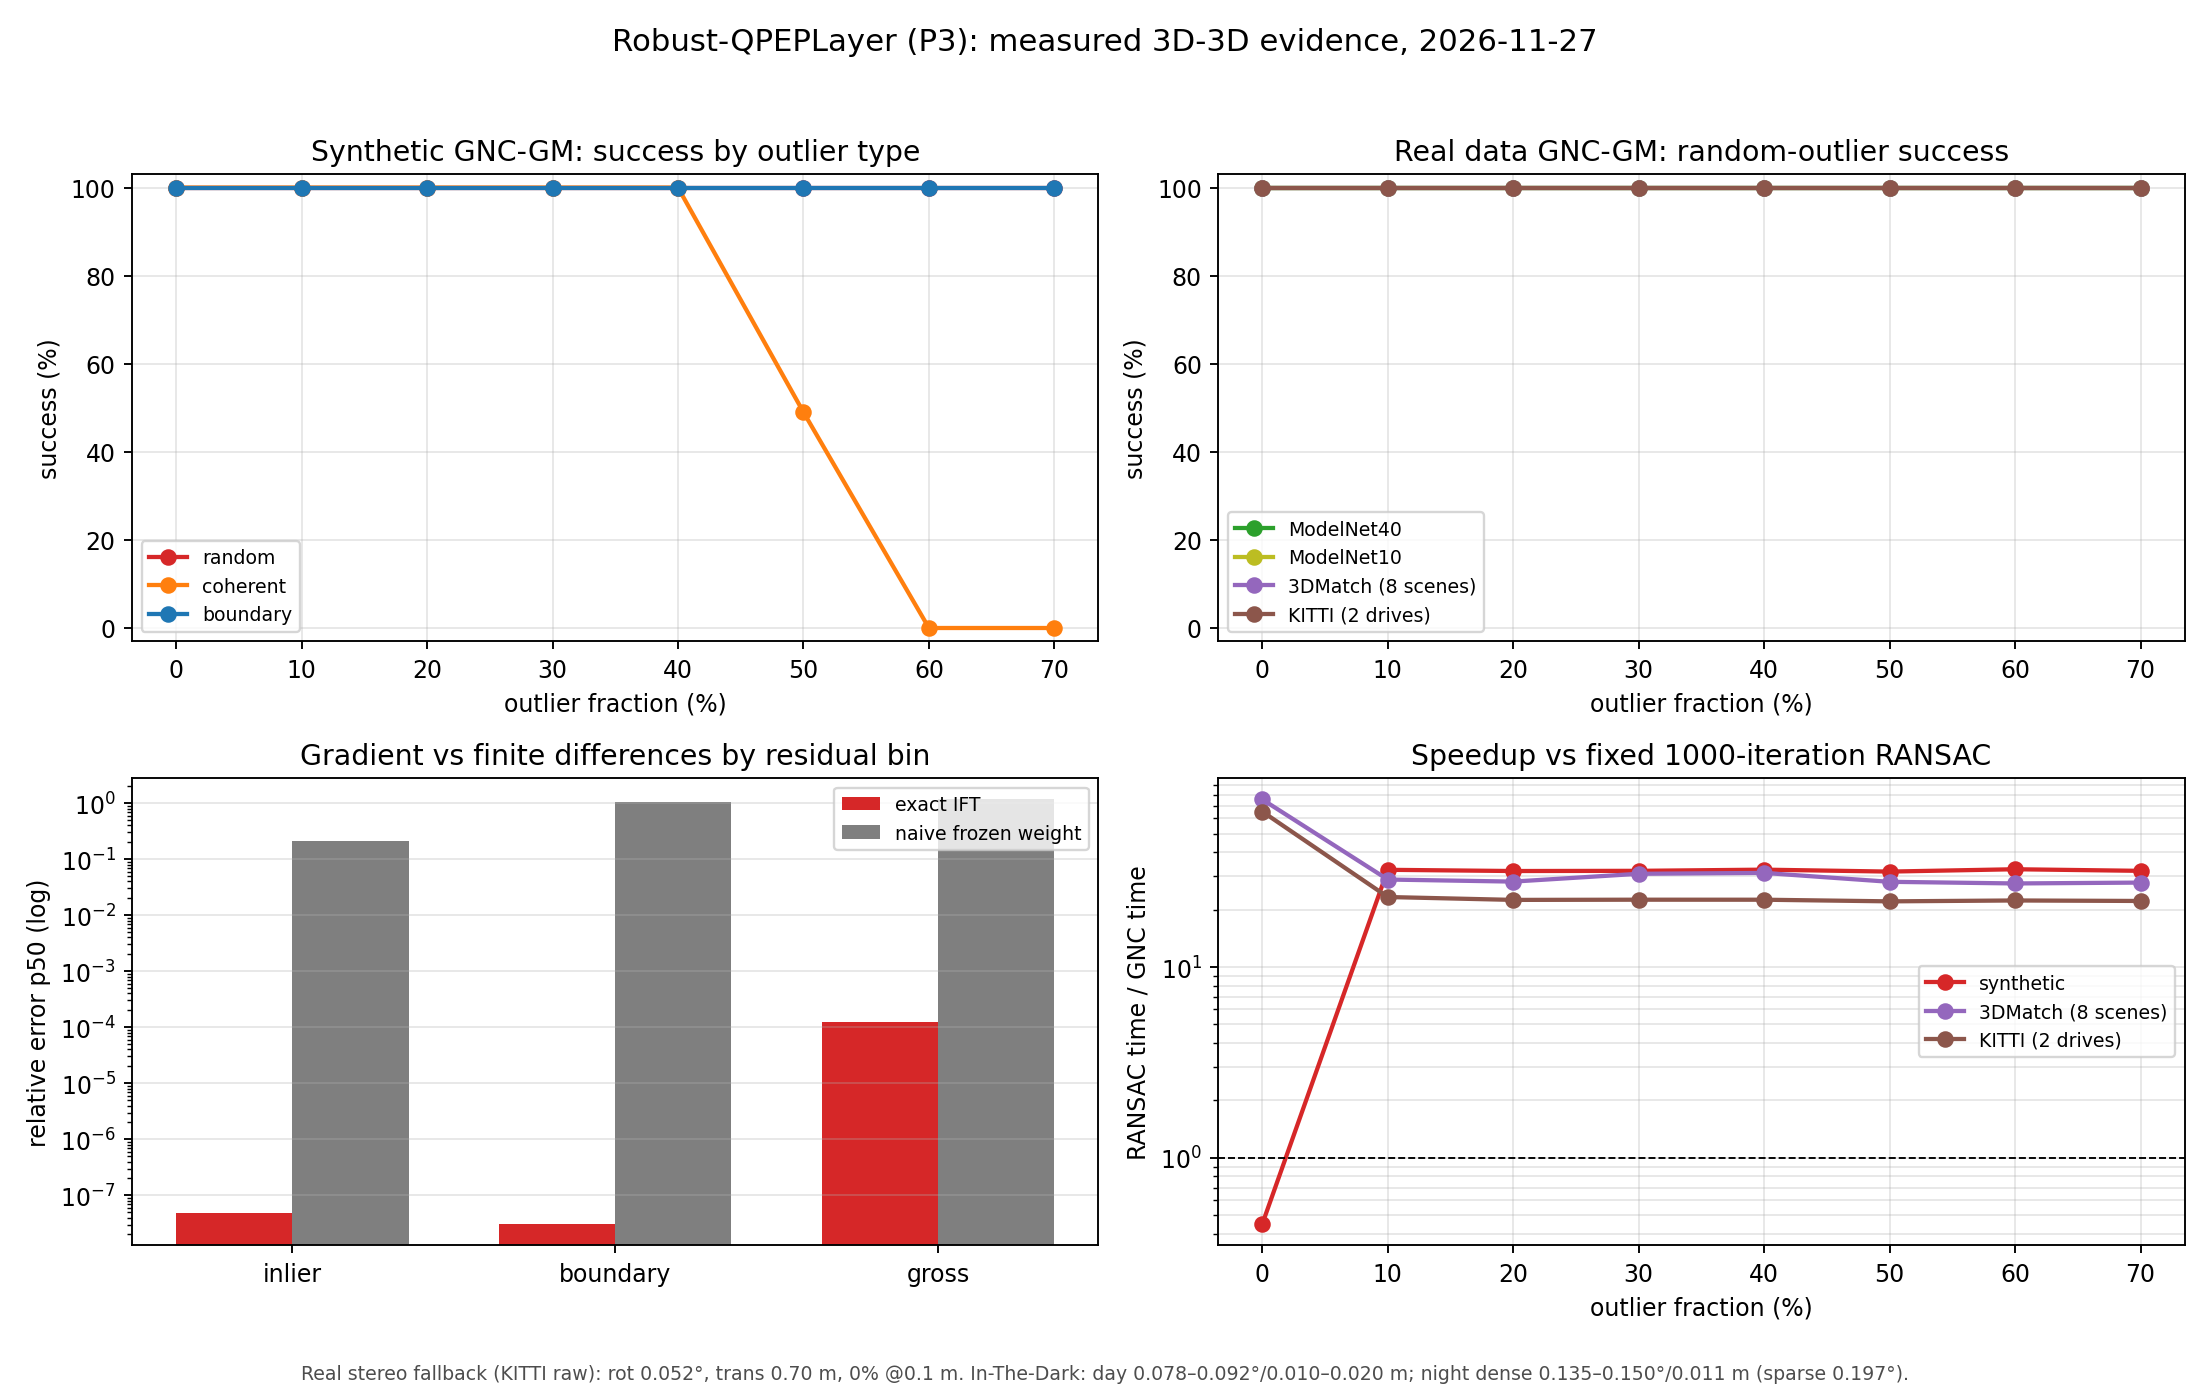
\includegraphics[width=\textwidth]{p3_summary.png}
\caption{Measured 3D--3D evidence (2026-11-27). (a) Synthetic GNC-GM success versus outlier
fraction for random, coherent, and boundary outliers: random and boundary stay at $100\%$,
coherent collapses once the outlier transform becomes the global optimum. (b) Real-data
random-outlier success for ModelNet40, ModelNet10, 3DMatch (8 scenes), and KITTI (2 drives); all
stay at $100\%$ through $70\%$. (c) 6D Jacobian relative error (p50, log scale) of exact IFT
versus naive frozen weights, by residual bin; the boundary bin is where freezing fails. (d)
GNC p50 runtime advantage over \emph{fixed-1000} RANSAC on synthetic, 3DMatch, and KITTI data; the
dashed line is break-even. The footer reports the KITTI stereo fallback and the In-The-Dark
day/night ranges. Success is rotation $<5^\circ$ and translation $<0.1$~m; source:
\texttt{experiments/make\_summary\_figure.py}.}
\label{fig:summary}
\end{figure*}

\section{Discussion and Limitations}
\label{sec:discussion}

\noindent\textbf{Limitations and future work.} The layer differentiates a local robust fixed point:
the outer GNC is not a global solver, provides no breakdown-point guarantee, and a coherent
majority of outliers can make the robust global optimum itself wrong. External baselines
(Theseus-GM and SDPRLayers+SCS) are evaluated on synthetic 3D--3D data, the real-data front ends are
hand-written (SIFT+StereoSGBM and FPFH), the night In-The-Dark evidence uses 10-pair windows, and no
learned descriptors are used. Extending the evaluation to learned front ends, real-data external
baselines, and full night sequences is the natural next step; a general 40-root QPEP inner solver
and GPU batching are left to future work.

\noindent\textbf{Model breakdown.} Even a perfect global solver for $F_{\mathrm{rob}}$ can return
the wrong pose when coherent outliers outnumber inliers. A one-dimensional example with one inlier
at $0$ and two coherent outliers at $M$ has $F(0)\to2c^2$ and $F(M)\to c^2$ as $M\to\infty$, so the
global minimum is the outlier pose. This identifiability limit calls for a consensus check, an
inlier-count diagnostic, or a prior on the outlier fraction.

\noindent\textbf{Boundary residuals.} $\lambda_\parallel$ is most negative at $e=c^2$, not at
$e\to\infty$. Gross outliers are suppressed at $O(\|\mathbf{r}\|^{-4})$, but a point just beyond the
redescending threshold has the largest gradient influence, so boundary residuals are both the most
sensitive part of training and the regime where the curvature correction matters most.

\noindent\textbf{Runtime against RANSAC.} RANSAC is a strong, well-tuned baseline, and the layer
removes its non-differentiable wrapper at the cost of a local robust estimator. Against fixed-budget
RANSAC the speedup is $22$--$32\times$; against adaptive-budget RANSAC the layer is slower at low
outlier fractions, at parity near $40\%$, and about $8\times$ faster at $70\%$; LO-RANSAC ties
accuracy but is $1.03$--$1.52\times$ slower than adaptive RANSAC, so the comparison is meaningful
only with the iteration budget stated.

\noindent\textbf{Kernel scale and residual model.} The framework covers GM, Cauchy, Welsch, and TLS,
but the scale $c$ is critical: a fixed $c$ may fail under varying noise, and a learned $c$ requires
a normalization such as $\det W_i=1$. The derivations are exact for residuals affine in
$\mathbf{t}$ and quadratic in the lifted quaternion; reprojection error is not polynomial and QPEP
uses an algebraic surrogate.

\noindent\textbf{Practical scope.} The layer fits when matches contain gross outliers, end-to-end
gradients through the pose are required, the outlier fraction is below the breakdown regime, and a
$6\times6$ backward with a fixed-size algebraic forward fits the budget; certified global solvers
remain preferable when global optimality is the objective.

\section{Conclusion}
\label{sec:conclusion}

We presented Robust-QPEPLayer, a RANSAC-free differentiable pose layer that combines BR duality,
GNC, and a constant-size QPEP inner solver, and differentiates the robust fixed point exactly. The
theory isolates two terms that the natural implementation drops: the redescending curvature
correction, which is the Schur complement of the BR weight block, and the constraint-multiplier term
of the unit-quaternion constraint. The one-dimensional sign-flip proposition gives a rigorous
setting in which the frozen-weight gradient has the wrong sign, and the per-observation
$O(\|\mathbf{r}\|^{-4})$ bound quantifies when the gradient through a gross outlier becomes
negligible. The method is not a global robust solver and does not replace RANSAC in adversarial
regimes; it is a principled, constant-dimension, exactly differentiable robust layer whose failure
modes are stated. Measured on synthetic data, ModelNet40/10, all eight official 3DMatch test scenes,
two KITTI raw drives, all 11 KITTI odometry sequences 00--10, and two daylight plus two night-prefix
In-The-Dark runs, it matches fixed-budget RANSAC success through $70\%$ random outliers at
$22$--$32\times$ lower runtime; that speedup does not hold against adaptive RANSAC at low outlier
fractions, and the exact gradient is $3$--$5\times10^{-8}$ relative to finite differences. Theseus-GM
and SDPRLayers+SCS are measured on synthetic data, but the full real-data external-baseline suite and
full-night/trained In-The-Dark pipeline remain future work; the KITTI stereo fallback is a
rotation-positive / translation-negative result, not a substitute.


\balance
\bibliographystyle{IEEEtran}
\bibliography{refs}

% ---------------------------------------------------------------- appendix
% Not counted toward the seven-page main-text limit. The \newpage makes the
% boundary explicit so the page number of the appendix start is the main-text
% page count (checked with \pageref{app:start}).
\newpage
\appendix
\section*{Appendix: Detailed Results}
\label{app:start}

This appendix collects proof and algorithm detail, the kernel-dual table, the per-dataset and
per-scene numbers behind Table~\ref{tab:real}, and the systems, baseline, and ablation detail.

\subsection*{A. Proofs, derivation notes, and the backward algorithm}
\label{app:proofs}
\label{app:backward}

The complete proofs of Lemmas~\ref{lem:brdual}--\ref{lem:weights},
Theorems~\ref{thm:gnc}--\ref{thm:rhs}, Propositions~\ref{prop:signflip}--\ref{prop:bound}, the
Schur-complement identity, the Riemannian Hessian formula, and the existence construction are
maintained in the project theory notes (\texttt{theory/proofs.md} and
\texttt{theory/derivations.md}); numerical checks are in \texttt{verify/}. The main text states the
results and the proof sketches; in particular:

\begin{itemize}
\item \emph{Lemma~\ref{lem:brdual}}: $w\mapsto we+\psi_\mu(w)$ is strictly convex on $(0,1]$ with
  stationary point $w^*$; substituting $w^*$ recovers $\rho_\mu(e)$, and the box constraint is a
  Cartesian product, so the multi-observation minimum is separable.
\item \emph{Lemma~\ref{lem:schur}}: differentiating the joint objective in $(z,w)$ gives $H_J$;
  eliminating $\delta w$ with $\psi''(w_i^*)=-1/\rho''(e_i^*)>0$ gives
  $H_{\mathrm{rob}}=H_{\mathrm{IRLS}}+\Delta H_{\mathrm{redesc}}$.
\item \emph{Lemma~\ref{lem:hessian}}: for $f\in C^2(\mathcal{M})$ the Euclidean Hessian restricted
  to the tangent space differs from the Riemannian Hessian by the second fundamental form, which for
  the unit sphere contributes $-(\mathbf{q}^\top G_q)\diag(I_4,0_3)$ \cite{absil2008}. For 3D--3D,
  $g_{i,q}^E=2J_i^\top W_i\mathbf{r}_i$ and $J_i\mathbf{q}=2\mathbf{u}_i$, hence
  $\lambda_i=\mathbf{q}^\top g_{i,q}^E=4\mathbf{u}_i^\top W_i\mathbf{r}_i$. The $W_i(\theta)$
  extension adds $2\mathbf{r}_i^\top(\partial W_i/\partial\theta)\mathbf{r}_i$ to
  $\partial e_i/\partial\theta$ and leaves the Hessian at fixed $W_i$ unchanged.
\item \emph{Proposition~\ref{prop:existence}}: the sign of
  $\Phi(t)=\sum_i2\rho'(e_i)(t-y_i)$ is evaluated at $t=0$ and $t=Kc^4/d^3$ for $d=y_2-y_1$, with
  $H_{\mathrm{rob}}\to\lambda_\parallel(0)=2>0$ as $d\to\infty$.
\item \emph{Proposition~\ref{prop:bound}}: the constants follow from
  $\|\partial\Phi/\partial\mathbf{y}_i\|_F\le Cc^4/(c^2+e_i)^2$,
  $\lambda_{\min}(H_{\mathrm{rob}})\ge\mu_0$, $\|\mathbf{r}_i\|^2=e_i$ for $W_i=I$, and
  $\|\rho'(e_i)g_i\|\le2\overline wc^4/\|\mathbf{r}_i\|^3$.
\end{itemize}

\begin{algorithm}[t]
\caption{Exact backward pass (implicit differentiation of the robust fixed point)}
\label{alg:backward}
\footnotesize
\begin{algorithmic}[1]
\Require upstream gradient; cached $z^*,w^*,e^*$
\For{$i=1$ to $N$}
  \State compute $\mathbf{u}_i,\mathbf{r}_i,J_i,g_i^E\in\mathbb{R}^7,H_i^E\in\mathbb{R}^{7\times7}$
\EndFor
\State $G\gets\sum_i\rho'_i g_i^E$;\quad
       $H_E\gets\sum_i\big(\rho'_iH_i^E+\rho''_ig_i^Eg_i^{E,\top}\big)$
\State $B_q\gets$ orthonormal basis of $\mathbf{q}^{*\perp}$;\quad $B\gets\diag(B_q,I_3)$
\State $H_{\mathrm{rob}}\gets B^\top H_EB-\lambda_{\mathrm{rob}}\diag(I_3,0_3)$,\quad
       $\lambda_{\mathrm{rob}}=\mathbf{q}^{*\top}G_q$
\State $\mathrm{RHS}\gets\sum_i\rho'_i\,\mathrm{d}g_i/\mathrm{d}\theta
       +\sum_i\rho''_ig_i(\mathrm{d}e_i/\mathrm{d}\theta)^\top$
\State $\mathrm{d}z\gets\mathrm{solve}(H_{\mathrm{rob}},-\mathrm{RHS})$
\State chain $\mathrm{d}z$ back to $(\mathbf{q},\mathbf{t})$ and to the upstream loss
\end{algorithmic}
\end{algorithm}

\begin{figure}[t]
\centering
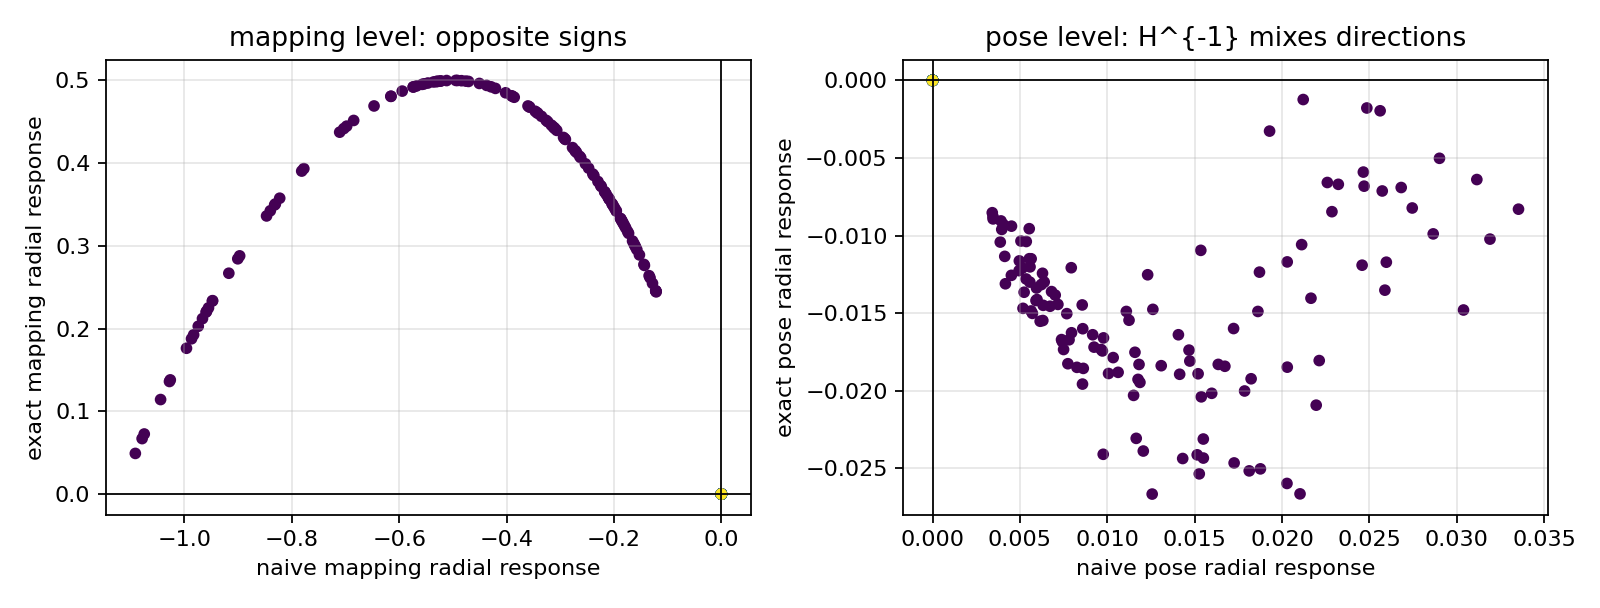
\includegraphics[width=\columnwidth]{gradient_sign.png}
\caption{Numerical sign structure behind Proposition~\ref{prop:signflip}. Left: mapping-level radial
response, exact versus frozen-weight (naive); for $e>c^2/3$ the signs are opposite. Right: pose-level
response after $H_{\mathrm{rob}}^{-1}$; the inverse Hessian mixes directions, so the 6D sign is
numerical.}
\label{fig:sign}
\end{figure}

\subsection*{B. Kernel duals}
\label{app:kernel}

Table~\ref{tab:kernel} lists the BR duals used by the layer, with $a=\mu c^2$. The forward and
backward passes are structurally identical across kernels: only $\rho_\mu'$ and $\psi_\mu''$ change.
TLS has a linear $\psi$ and a non-unique weight at $e=a$; it requires the GNC-TLS schedule rather
than plain bandwidth annealing.

\begin{table}[t]
\caption{Black--Rangarajan duals for the four kernels ($a=\mu c^2$).}
\label{tab:kernel}
\centering
\scriptsize
\setlength{\tabcolsep}{1.4pt}
\begin{tabular}{llll}
\toprule
kernel & $\rho_\mu(e)$ & $w^*=\rho_\mu'(e)$ & $\psi_\mu(w)$ \\
\midrule
Geman--McClure & $ae/(a+e)$ & $(a/(a+e))^2$ & $a(\sqrt{w}-1)^2$ \\
Cauchy & $a\log(1+e/a)$ & $a/(a+e)$ & $a(w-1-\log w)$ \\
Welsch & $a(1-e^{-e/a})$ & $e^{-e/a}$ & $a(1-w+w\log w)$ \\
TLS & $\min(e,a)$ & $1$ if $e<a$, $0$ if $e>a$ & $a(1-w)$ \\
\bottomrule
\end{tabular}
\end{table}

\subsection*{C. Per-dataset results}
\label{app:datasets}

\noindent\textbf{ModelNet40/10.} Table~\ref{tab:modelnet} gives the aggregate numbers. ModelNet10
uses 908 test objects in 10 classes, with OFF meshes resampled to 2048 points; robust-method success
differs from ModelNet40 by at most $2$~pp and median rotation by at most $0.038^\circ$. GNC runs in
$1.7$--$1.9$~ms versus $53.5$--$61.5$~ms for fixed-1000 RANSAC on both datasets.

\begin{table}[t]
\caption{ModelNet object-cloud results under uniform random outliers, 50 trials/cell, $N=100$,
$c=0.05$~m. Entries are success rates; ``fail'' marks collapse.}
\label{tab:modelnet}
\centering
\scriptsize
\setlength{\tabcolsep}{2.5pt}
\begin{tabular}{lcccc}
\toprule
dataset & GNC & RANSAC-1000 & IRLS & Kabsch \\
\midrule
ModelNet40 & $100\%$ $\le70\%$ & $100\%$ & $98$--$100\%$ & fail $\ge50\%$ \\
ModelNet10 & $100\%$ $\le70\%$ & $100\%$ & $98$--$100\%$ & fail $\ge50\%$ \\
\bottomrule
\end{tabular}
\end{table}

\noindent\textbf{3DMatch.} Table~\ref{tab:3dmatch} gives the pooled eight-scene row, the
low/mid/high overlap study, the stricter $0.20$--$0.50$ band, and the two FPFH-front-end audits.
Pooled over all eight official test scenes (20 trials/cell), GNC p50 at $p=0.7$ is $2.26$~ms vs
$62.6$~ms for fixed-1000 RANSAC ($27.7\times$), and the boundary median rotation at $p=0.7$ is
$0.27^\circ$ vs $0.52^\circ$. Per-scene GNC p50 is $2.26$--$2.36$~ms vs $62.1$--$73.4$~ms
($27.4$--$31.1\times$), IRLS is $99\%$ at $70\%$, and coherent outliers collapse at $60$--$70\%$ for
every method ($0\%$). The overlap study selects 24/21/20 pairs for the high/mid/low bins; clean
rotation is $0.18^\circ$/$0.24^\circ$/$0.52^\circ$, yet GNC and RANSAC both stay at $100\%$ at
$p=0.7$ in every bin, with a zero success delta and a $27.7$--$30.4\times$ speedup for $p\ge30\%$.
The low bin still has a median base inlier fraction of $0.95$. The stricter $0.20$--$0.50$
geometric-overlap band (4 low + 2 matched high pairs per scene, 10 trials/cell) has oracle base
inlier $0.953$ (low) / $0.984$ (high) and clean rotation $0.47^\circ$ / $0.19^\circ$; GNC and
RANSAC-1000 are $100\%$ at $p=0.7$, IRLS $92\%$, Kabsch $1\%$. Low overlap reduces the \emph{number}
of usable correspondences, not the oracle inlier fraction. The FPFH front-end (mutual NN plus
pairwise-distance consistency, no GT in matching) reaches natural inlier rates of $80.0\%$ and
$67.8\%$ on the two audited scenes.

\begin{table*}[t]
\caption{3DMatch detail. Oracle correspondences use GT-mapped nearest neighbours on real overlapping
fragments; FPFH rows use a hand-crafted front-end with no GT in matching. ``bnd'' = boundary
outliers.}
\label{tab:3dmatch}
\centering
\scriptsize
\setlength{\tabcolsep}{2.2pt}
\begin{tabular}{lcccccc}
\toprule
setting & pairs/trials & clean rot & GNC & RANSAC-1000 & Kabsch & speedup \\
\midrule
pooled 8 test scenes, random & 8 pairs/scene, 20 trials/cell & --- & $100\%$ $\le70\%$ & $100\%$ & --- & $27.7\times$ @$70\%$ \\
pooled 8 test scenes, bnd.\ @$70\%$ & 8 pairs/scene, 20 trials/cell & --- & $0.27^\circ$ & $0.52^\circ$ & --- & --- \\
overlap high & 24 pairs & $0.18^\circ$ & $100\%$ @$0.7$ & $100\%$ & --- & $27.7$--$30.4\times$ \\
overlap mid & 21 pairs & $0.24^\circ$ & $100\%$ @$0.7$ & $100\%$ & --- & $27.7$--$30.4\times$ \\
overlap low & 20 pairs & $0.52^\circ$ & $100\%$ @$0.7$ & $100\%$ & --- & $27.7$--$30.4\times$ \\
strict $0.20$--$0.50$ band & 4 low + 2 high pairs/scene, 10 trials/cell & $0.47^\circ$ / $0.19^\circ$ & $100\%$ @$0.7$ & $100\%$ & $1\%$ & --- \\
FPFH audit 1 & natural inliers $80.0\%$ & --- & $100\%$ & $100\%$ & $100\%$ & --- \\
FPFH audit 2 & natural inliers $67.8\%$ & --- & $100\%$ & $97\%$ & $83\%$ & --- \\
\bottomrule
\end{tabular}
\end{table*}

\noindent\textbf{KITTI.} Table~\ref{tab:kitti} collects the raw-drive and odometry rows. For the raw
drives, ego motion comes from OXTS (Mercator + roll/pitch/yaw) mapped to Velodyne with
\texttt{calib\_imu\_to\_velo}; direction is verified (drive 0001 correct NN $0.100$--$0.123$~m vs
inverse $0.143$--$0.183$~m; drive 0002 $0.108$--$0.140$~m vs $0.136$--$0.269$~m). Drive 0002
reproduces the drive-0001 random and boundary tables exactly, keeps the coherent transition (at
$50\%$ GNC $40\%$ vs $35\%$, IRLS $30\%$ vs $45\%$; both chance-level), and gives the
$\sim21$--$23\times$ speedup. A threshold sweep keeps GNC at $100\%$ for
$c\in\{0.15,0.25,0.35\}$, with $c=0.25$ matching the $\sim0.10$~m point spacing. For odometry, only
the 32--33 touched frames per sequence were range-fetched from the 84.8~GB official archive, so all
11 sequences 00--10 are represented. On the eight added sequences (10 trials/cell) success is
$100\%$ for GNC and RANSAC-1000 at $p=0.7$ except seq~08 ($80\%$ at $p=0$ and $p=0.3$; RANSAC
$100\%$); pooled over 11 sequences success is $99/99/100/100\%$ at $p=0/0.3/0.5/0.7$, and the
fixed-RANSAC/GNC runtime ratio is $22.4\times$ at $p\ge0.3$. The 00/05/07 subset gives the
failure-mode detail: all 18 direction checks pass (fwd NN $0.053$--$0.114$~m vs inverse
$0.104$--$0.430$~m), random success is $100\%$ through $70\%$, pooled GNC $2.8$~ms vs $73.7$~ms
($26.3\times$), coherent collapse at $p=0.6$ (at $p=0.5$ GNC $53\%$, IRLS $38\%$, RANSAC $0\%$),
boundary $0.067^\circ$ vs $0.143^\circ$, and across $|\mathbf{t}|=0.09$--$9.62$~m and gaps
$1/2/4/8$ (171 paired cells) GNC is never below RANSAC. The exact-pose clean floor
($0.042$--$0.057^\circ$) is not lower than the OXTS raw drives ($0.030$--$0.039^\circ$), so LiDAR
sampling/voxelization dominates it.

\begin{table*}[t]
\caption{KITTI raw drives and odometry, $N=300$, $c=0.25$~m, 20 trials/cell (added sequences 10
trials/cell). Random-outlier success is $100\%$ for GNC and fixed-1000 RANSAC through $70\%$ except
seq~08.}
\label{tab:kitti}
\centering
\footnotesize
\setlength{\tabcolsep}{3pt}
\begin{tabular}{lcccccc}
\toprule
sequence & frames/pairs & GNC p50 & RANSAC p50 & speedup & coh.\ @$50\%$ & bnd.\ rot \\
\midrule
raw 0001 & 108 frames, 10 pairs & $2.7$--$2.8$~ms & $61$--$64$~ms & $\sim22\times$ & $0\%$ all & $0.07$--$0.09^\circ$ \\
raw 0002 & 77 frames, 10 pairs & $2.7$--$2.8$~ms & $61$--$64$~ms & $\sim21$--$23\times$ & $40/35/30/45\%$ & $0.07$--$0.09^\circ$ \\
odom 00--10 & 33 frames each, pooled & $2.8$~ms & $73.7$~ms & $22.4\times$ & seq~08 $80\%$ @$p\le0.3$ & --- \\
odom 00/05/07 & 33 frames each & $2.8$~ms & $73.7$~ms & $26.3\times$ & $53/38/0\%$ & $0.067/0.143^\circ$ \\
\bottomrule
\end{tabular}
\end{table*}

\noindent\textbf{In-The-Dark.} Table~\ref{tab:inthedark} gives the daylight runs and the night
windows. The composed official GT was validated by stereo reprojection on disjoint pairs: forward
medians $0.65$~px (run\_000002) and $0.52$~px (run\_000012), versus $18.1/27.9$~px inverse,
$9.5/14.7$~px identity, and $21.5/31.3$~px unconjugated. All checks pass (512$\times$384 images,
left/right row alignment $0.56$--$0.58$~px). The archive is 905~MB but only the 315{,}463-byte
transform file was range-fetched (CRC verified); the night zips (2.6--2.76~GB) were not downloaded,
and only the touched windows were fetched. The motion-matched daylight control (run\_000002 start
757, $|\mathbf{t}|=0.21$~m, rot $0.54^\circ$) gives $85.9\%$ inliers and $0.121^\circ/0.007$~m;
median depth is $4.5$~m at night vs $6.7$--$7.2$~m by day, so the night inlier rate is a geometry
effect rather than a property of SIFT in low light.

\begin{table*}[t]
\caption{UTIAS In-The-Dark: two daytime runs (15 consecutive pairs each) and two night-window
prefixes (10 pairs each); hand-written SIFT+StereoSGBM front-end, no training. GT reprojection
columns are median px (fwd / inverse / identity / unconjugated vehicle frame).}
\label{tab:inthedark}
\centering
\footnotesize
\setlength{\tabcolsep}{3pt}
\begin{tabular}{llcccccc}
\toprule
run & pairs & inliers & rot & trans & succ.\ @$0.1$~m & Kabsch & GT reproj \\
\midrule
day run\_000002 & 15 & $79.4\%$ & $0.078^\circ$ & $0.020$~m & $100\%$ & $47\%$ & $0.65/18.1/9.5/21.5$ \\
day run\_000012 & 15 & $88.5\%$ & $0.092^\circ$ & $0.010$~m & $100\%$ & $40\%$ & $0.52/27.9/14.7/31.3$ \\
night run\_000017 & 10 & $96.0\%$ & $0.135^\circ$ & $0.011$~m & $100\%$ & --- & --- \\
night run\_000018 & 10 & $97.1\%$ & $0.150^\circ$ & $0.011$~m & $100\%$ & --- & --- \\
night sparse & 10 & $84.3\%$ & $0.197^\circ$ & $0.015$~m & --- & --- & --- \\
day control & 10 & $85.9\%$ & $0.121^\circ$ & $0.007$~m & --- & --- & --- \\
\bottomrule
\end{tabular}
\end{table*}

\noindent\textbf{KITTI stereo front end.} Thirty frame pairs of drive 0001 with SIFT + sub-pixel +
StereoSGBM on rectified \texttt{image\_02/03} ($b=0.5327$~m) give a natural inlier rate of $17.8\%$
at $c=0.5$~m with 890 correspondences/pair. GNC/IRLS recover rotation to $0.052^\circ$ against a
GT-inlier floor of $0.071^\circ$, but translation is $0.70$~m median versus $1.92$~m motion and a
$0.239$~m floor; no method attains $0.1$~m or $0.25$~m success. GNC is $19.3\times$ faster than
fixed-1000 RANSAC (4.21 vs 81.3~ms). The stereo-vs-LiDAR depth ratio is $1.000$--$1.061$ over
3--60~m, ruling out a disparity-scale error; the residual is a coherent forward-translation
under-estimate ($0.63$--$0.73$) from front-end, occlusion, and dynamic bias.

\subsection*{D. Systems, batching, and the inner solver}
\label{app:systems}

A vectorized NumPy GNC over $(B,N,3)$ reproduces the loop to rotation $\le1.1\times10^{-14}$ and
translation $\le1.2\times10^{-15}$ with identical $\mu$-schedules. At $B=32,N=100$ the batch p50 is
$8.5$~ms vs $56.2$~ms for the loop ($6.60\times$); at $B=8$ the speedup is $2.95\times$ ($N=100$)
and $3.27\times$ ($N=500$); $B=1$ is slower ($0.54\times$), so the loop remains the right choice for
single instances.

A $4\times4$ Davenport/Horn inner solver \cite{horn1987} is numerically equivalent to weighted
Kabsch (max $\|R_d-R_k\|_F=1.07\times10^{-14}$, max cost excess $9.4\times10^{-16}$) but its
runtime is better only at large $N$: p50 ratio $0.94\times$ ($N=20$), $1.02\times$ ($N=100$),
$1.28\times$ ($N=500$), geometric mean $1.07\times$. It is a large-$N$ option rather than a
default $N=100$ gain.

\subsection*{E. External baselines (synthetic only)}
\label{app:baselines}

Theseus 0.2.3 (dense Cholesky; \texttt{scikit-sparse} unavailable without SuiteSparse headers)
solves the same per-point GM objective; its Jacobian matches finite differences at
$1.09\times10^{-10}$ relative error and its GM cost agrees exactly. With GT initialization Theseus-GM
succeeds $100\%$ at all $p$ (a local-basin check, not global recovery); with random initialization it
succeeds $100/80/55/25\%$ at $p=0/0.3/0.5/0.7$, p50 $358$--$670$~ms. On the same 20 instances GNC-GM
is $100\%$ at every $p$ at $1.7$~ms, RANSAC-adaptive is $100\%$ at $0.2$--$14.1$~ms, and Kabsch
fails for $p\ge0.3$. The 20-trial Wilson intervals for Theseus random-init at $p=0.3$
([0.58,0.92]) overlap GNC's 20/20 ([0.84,1.00]), so that gap is not significant; $p=0.5/0.7$ are
separated (Table~\ref{tab:baselines}).

\begin{table}[t]
\caption{Synthetic external baselines, 20 instances per $p$; success (\%) at $p=0/0.3/0.5/0.7$ and
p50 time.}
\label{tab:baselines}
\centering
\footnotesize
\setlength{\tabcolsep}{3pt}
\begin{tabular}{lcccc}
\toprule
method & $p=0$ & $0.3$ & $0.5$ & $0.7$ / time \\
\midrule
Theseus-GM, GT init & 100 & 100 & 100 & 100 \\
Theseus-GM, rand.\ init & 100 & 80 & 55 & 25 / 358--670~ms \\
GNC-GM & 100 & 100 & 100 & 100 / 1.7~ms \\
RANSAC-adaptive & 100 & 100 & 100 & 100 / 0.2--14.1~ms \\
Kabsch & 100 & fail & fail & fail \\
SDPRLayers+SCS & 100 & fail & fail & fail / 8.5--13.4~ms \\
\bottomrule
\end{tabular}
\end{table}

SDPRLayers+SCS (fresh \texttt{utiasASRL/sdprlayer} at cb3aed2, SCS, 208 forwards) is numerically
available: $0/208$ SCS exceptions, $8.5$--$13.4$~ms. It succeeds at $p=0$ but fails at $p\ge0.3$, as
expected without a robust kernel. With $W_i=I$ and unit weights its objective equals Kabsch: 80
paired trials give max $|\Delta R|=1.5\times10^{-5}$~deg and max $|\Delta t|=1.3\times10^{-9}$~m.
This row validates forward correctness and availability; a distinct SDPR requires non-identity
$W_i$ (e.g.\ POLI) or RANSAC. BPnP is 3D--2D PnP only, Pyatov \emph{et al.} is two-view 2D--2D, and
POLI is a per-point geometry estimator, so none is a direct 3D--3D baseline.

\subsection*{F. Ablations}
\label{app:ablations}

\noindent\textbf{Kernel.} With the same weighted-Kabsch inner and schedule, GM, Cauchy, and Welsch
are all $100\%$ on random and boundary outliers through $70\%$ (Table~\ref{tab:kernelabl}). GM has
the lowest boundary median rotation at $50$--$70\%$ ($0.199/0.229/0.340^\circ$ vs Cauchy
$0.241/0.264/0.370^\circ$ and Welsch $0.220/0.268/0.392^\circ$). There is no evidence to switch the
default.

\begin{table}[t]
\caption{Kernel ablation: boundary median rotation (deg) at $p=0.5/0.6/0.7$; all kernels are
$100\%$ on random and boundary outliers through $70\%$.}
\label{tab:kernelabl}
\centering
\footnotesize
\setlength{\tabcolsep}{4pt}
\begin{tabular}{lccc}
\toprule
kernel & $p=0.5$ & $p=0.6$ & $p=0.7$ \\
\midrule
GM (default) & $0.199$ & $0.229$ & $0.340$ \\
Cauchy & $0.241$ & $0.264$ & $0.370$ \\
Welsch & $0.220$ & $0.268$ & $0.392$ \\
\bottomrule
\end{tabular}
\end{table}

\noindent\textbf{GNC schedule.} Sweeping $\gamma\in\{1.2,1.4,1.7,2.0\}$, the $\mu_0$ multiplier
$\{0.5,1,4\}$ and polish steps $\{0,5,10\}$ gives $100\%$ success and identical median rotation at
$p=0.3/0.5/0.7$; $\gamma=2.0$ is $1.04$--$1.79\times$ faster than the default, $\gamma=1.2$ is
$1.47$--$2.49\times$ slower. The default is conservative rather than uniquely optimal.

\noindent\textbf{RANSAC strength.} A stronger LO-RANSAC (MSAC score, up to five local refit/re-score
rounds, 0.999 adaptive stop, cap 1000) ties GNC on accuracy (median rotation difference
$\le0.006^\circ$) but is $1.03$--$1.52\times$ slower than plain adaptive RANSAC at every $p$, because
the final consensus refit is already the same estimator.

\noindent\textbf{Anisotropic $W_i$.} With a correct 6-DoF Gauss--Newton inner solve on
Cholesky-whitened residuals, $W_i=I$ matches Kabsch to $5.3\times10^{-13}$. Scalar weighted Kabsch
is not exact for anisotropic $W_i$: its objective ratio at converged GM weights is
$1.002$--$1.007$ (diagonal) and $1.035$--$1.088$ (full SPD), with a single-trial maximum of $3.80$.
Under the isotropic synthetic noise, however, anisotropic $W_i$ is a misspecified model: full-$W$
GNC has a paired median rotation change of $+0.055$ to $+0.124^\circ$, is better on only
$8$--$32\%$ of trials, and has $92\%$ success at $p=0.7$ (identity: $100\%$). The exact inner solve
is $4.9$--$23\times$ slower than scalar Kabsch. The nonlinear inner solve is therefore appropriate
when $W_i$ is genuinely anisotropic, while anisotropy does not improve accuracy on this isotropic
data.

\subsection*{G. End-to-end boundary diagnostic}
\label{app:e2e}

A GT-supervised test-time refinement updates only the injected boundary observations for 20 Adam
steps. At $p=0.5$, lr $10^{-3}$, the exact gradient reaches a final loss of $1.90\times10^{-6}$ vs
$1.66\times10^{-5}$ for naive (paired median ratio $0.071$, a $14\times$ reduction; exact lower on
$10/10$ seeds) and rotation error $0.029^\circ$ vs $0.087^\circ$; at $p=0.7$ the median ratio is
$0.059$ ($17\times$) and exact wins $9/10$. The all-points control is not discriminative
($4$--$9/10$, ratio $0.64$--$1.04$). A float64 PyTorch \texttt{autograd.Function} passes
\texttt{gradcheck} at $N=6/8/10$ and agrees with NumPy to $10^{-16}$ in pose; a per-point MLP
refinement (5 seeds, $p=0.4$, 50 Adam steps) reduces median rotation from $0.635^\circ$ to
$0.068^\circ$ for exact vs $0.106^\circ$ for naive (exact wins $4/5$ seeds, median loss ratio
$0.56$), while a disjoint held-out protocol overfits in both arms. This is a controlled test-bed for
the layer implementation rather than a trained real-data system.

The per-coordinate gradient check is exact to
$1.6\times10^{-7}$ / $3.9\times10^{-8}$ / $9.3\times10^{-8}$ relative error, versus $1.42$ / $0.60$ /
$0.38$ for the naive backward. The float64 PyTorch \texttt{autograd.Function} passes
\texttt{gradcheck} at $N=6/8/10$ with maximum absolute error $6$--$8\times10^{-10}$ and maximum
relative error $8\times10^{-9}$--$1.1\times10^{-8}$, except one near-zero element at
$8\times10^{-6}$; the naive backward fails at relative error $1.5$--$1.8$, and the torch port agrees
with NumPy to $10^{-16}$ in pose and $3\times10^{-16}$ in $\mathrm{d}L/\mathrm{d}\mathbf{y}$.

\begin{figure*}[t]
\centering
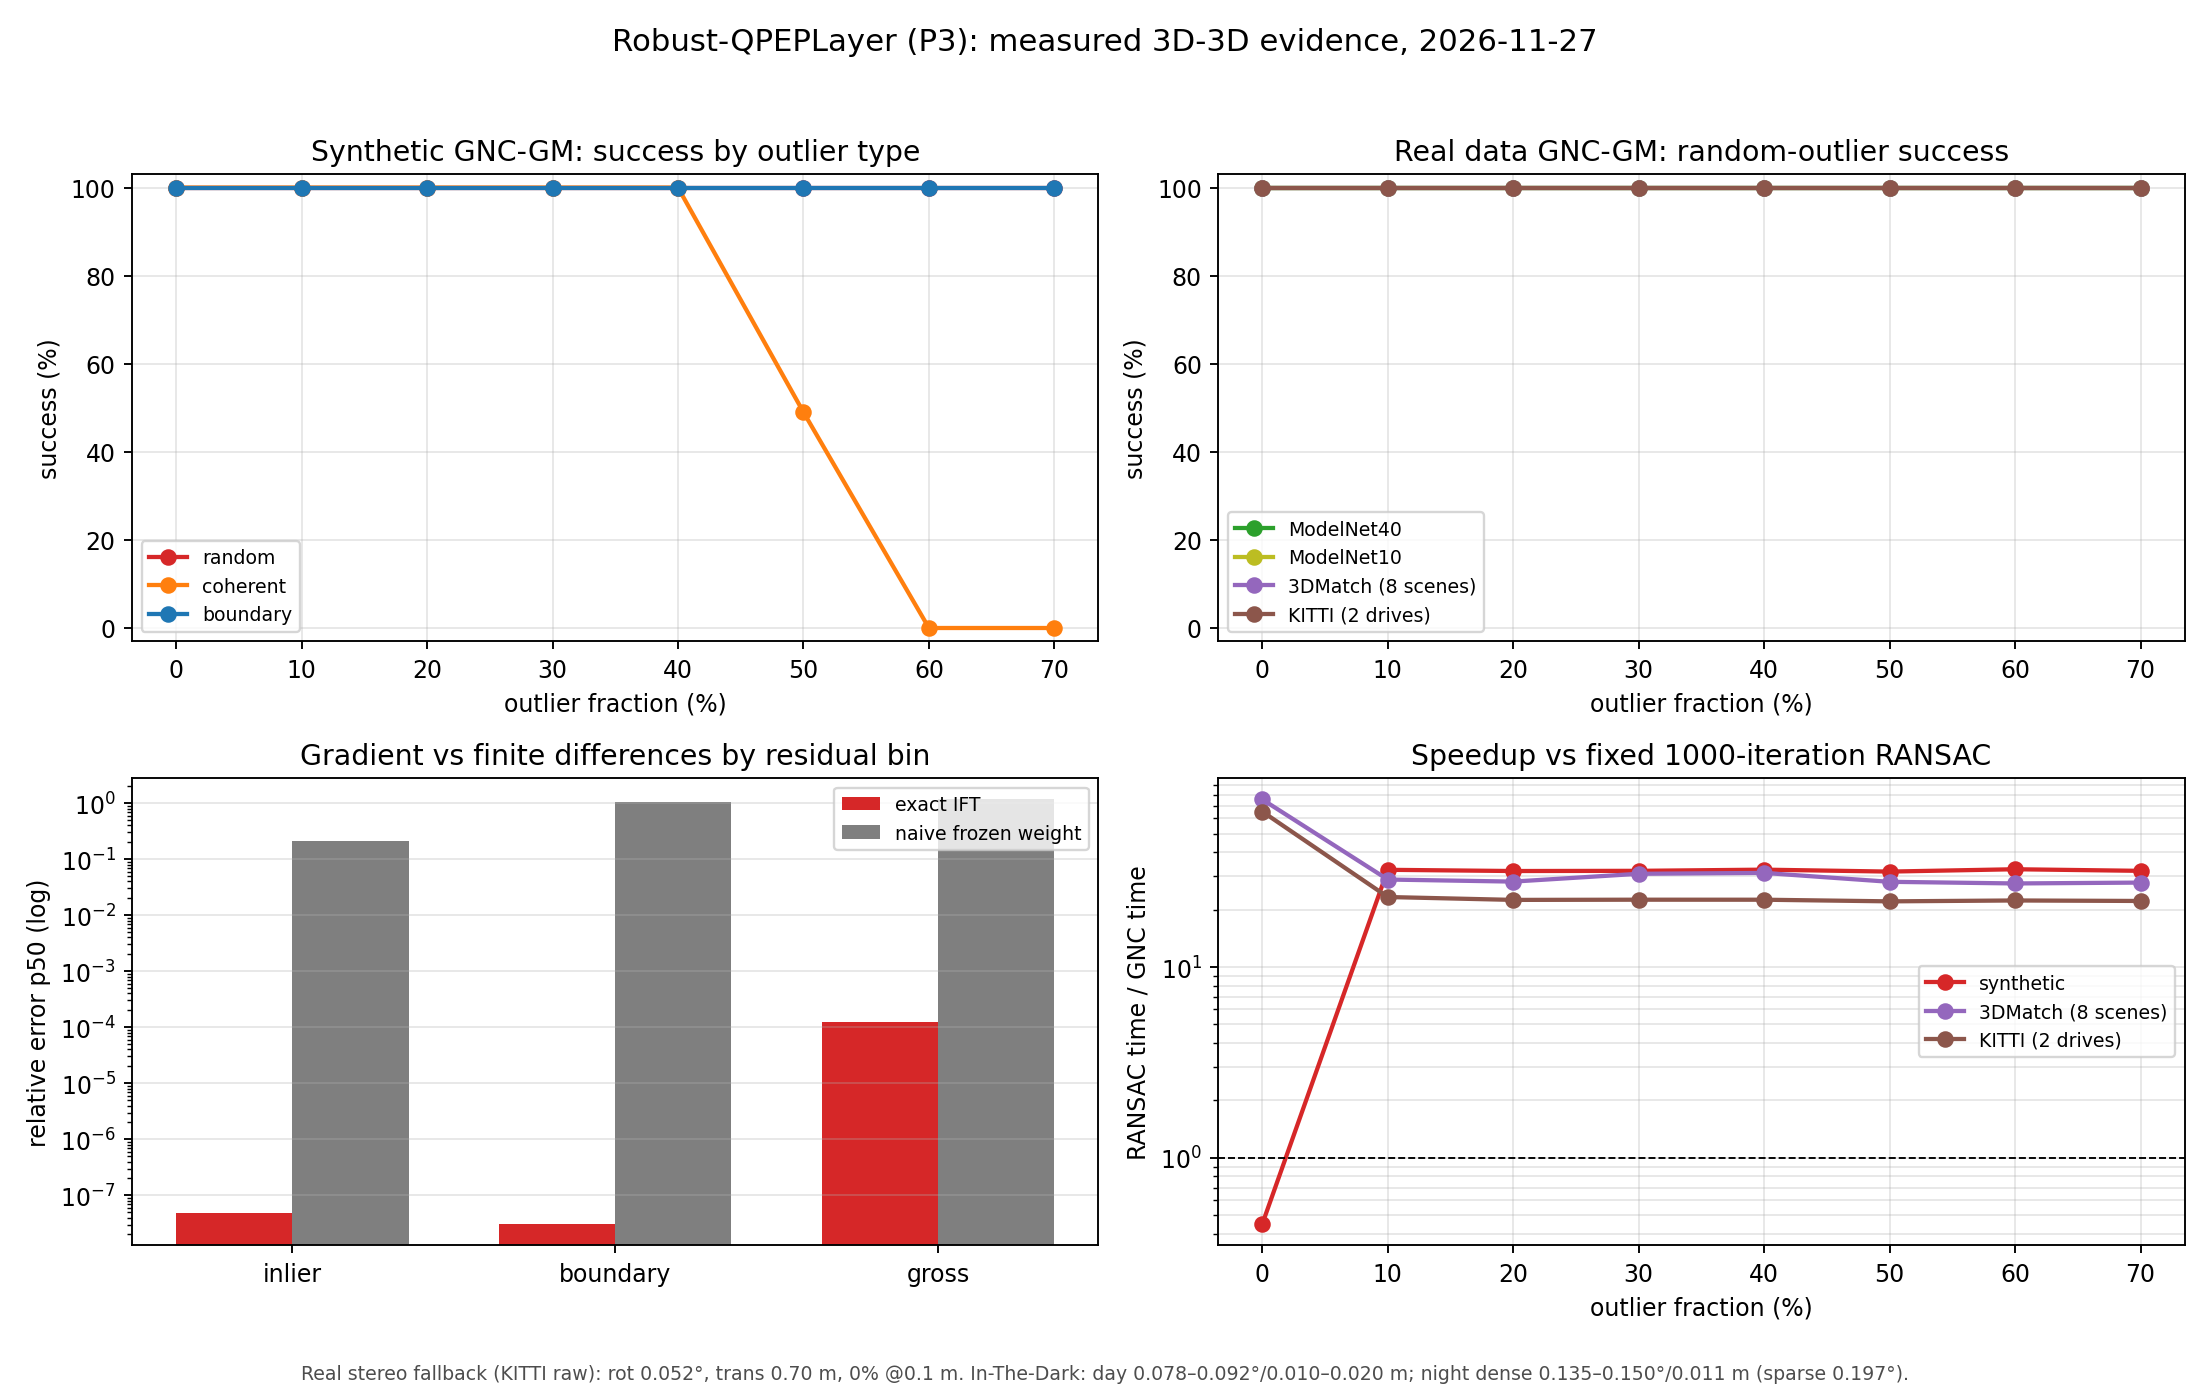
\includegraphics[width=0.92\textwidth]{p3_summary.png}
\caption{Measured 3D--3D evidence. (a) Synthetic GNC-GM success versus outlier fraction for random,
coherent, and boundary outliers: random and boundary stay at $100\%$, coherent collapses once the
outlier transform becomes the global optimum. (b) Real-data random-outlier success for ModelNet40,
ModelNet10, 3DMatch (8 scenes), and KITTI (2 drives); all stay at $100\%$ through $70\%$. (c) 6D
Jacobian relative error (p50, log scale) of exact IFT versus naive frozen weights, by residual bin;
the boundary bin is where freezing fails. (d) GNC p50 runtime advantage over \emph{fixed-1000}
RANSAC on synthetic, 3DMatch, and KITTI data; the dashed line is break-even. The footer reports the
KITTI stereo front end and the In-The-Dark day/night ranges. Success is rotation $<5^\circ$ and
translation $<0.1$~m.}
\label{fig:summary}
\end{figure*}


\end{document}
